\setlength\topmargin{8mm}
\onehalfspacing
\chapter{Programació del software} % Main chapter title

\label{Chapter5} % For referencing the chapter elsewhere, use \ref{Chapter1} 

\rhead[\emph{Disseny, programació i implementació d'un robot de dibuix amb Arduino}]{\thepage}
\lhead[\thepage]{\emph{Disseny, programació i implementació d'un robot de dibuix amb Arduino}}





\definecolor{mygreen}{rgb}{0,0.6,0}
\definecolor{mygray}{rgb}{0.47,0.47,0.33}
\definecolor{myorange}{rgb}{0.8,0.4,0}
\definecolor{mywhite}{rgb}{0.98,0.98,0.98}
\definecolor{myblue}{rgb}{0.01,0.61,0.98}

\newcommand*{\FormatDigit}[1]{\ttfamily\textcolor{mygreen}{#1}}
%% https://tex.stackexchange.com/questions/32174/listings-package-how-can-i-format-all-numbers
\lstdefinestyle{FormattedNumber}{%
	literate=*{0}{{\FormatDigit{0}}}{1}%
	{1}{{\FormatDigit{1}}}{1}%
	{2}{{\FormatDigit{2}}}{1}%
	{3}{{\FormatDigit{3}}}{1}%
	{4}{{\FormatDigit{4}}}{1}%
	{5}{{\FormatDigit{5}}}{1}%
	{6}{{\FormatDigit{6}}}{1}%
	{7}{{\FormatDigit{7}}}{1}%
	{8}{{\FormatDigit{8}}}{1}%
	{9}{{\FormatDigit{9}}}{1}%
	{.0}{{\FormatDigit{.0}}}{2}% Following is to ensure that only periods
	{.1}{{\FormatDigit{.1}}}{2}% followed by a digit are changed.
	{.2}{{\FormatDigit{.2}}}{2}%
	{.3}{{\FormatDigit{.3}}}{2}%
	{.4}{{\FormatDigit{.4}}}{2}%
	{.5}{{\FormatDigit{.5}}}{2}%
	{.6}{{\FormatDigit{.6}}}{2}%
	{.7}{{\FormatDigit{.7}}}{2}%
	{.8}{{\FormatDigit{.8}}}{2}%
	{.9}{{\FormatDigit{.9}}}{2}%
	%{,}{{\FormatDigit{,}}{1}% depends if you want the "," in color
	{\ }{{ }}{1}% handle the space
	,%
}


\lstset{%
	backgroundcolor=\color{mywhite},   
	basicstyle=\footnotesize,       
	breakatwhitespace=false,         
	breaklines=true,                 
	captionpos=b,                   
	commentstyle=\color{red},    
	deletekeywords={...},           
	escapeinside={\%*}{*)},          
	extendedchars=true,              
	%frame=shadowbox,                    
	keepspaces=true,                 
	keywordstyle=\color{myorange},       
	language=Octave,                
	morekeywords={*,...},            
	%numbers=left,                    
	%numbersep=5pt,                   
	%numberstyle=\tiny\color{mygray}, 
	rulecolor=\color{black},         
	rulesepcolor=\color{myblue},
	showspaces=false,                
	showstringspaces=false,          
	showtabs=false,                  
	%stepnumber=2,                    
	stringstyle=\color{myorange},    
	tabsize=2,                       
	title=\lstname,
	emphstyle=\bfseries\color{blue},%  style for emph={} 
}    

%% language specific settings:
\lstdefinestyle{Arduino}{%
	style=FormattedNumber,
	keywords={void, int, long, boolean, pinMode, digitalWrite},%                 define keywords
	morecomment=[l]{//},%             treat // as comments
	morecomment=[s]{/*}{*/},%         define /* ... */ comments
	emph={HIGH, OUTPUT, LOW},%        keywords to emphasize
}







En aquest capítol es presenta la programació del robot. Aquesta programació es basa principalment en dos grans blocs que actuen conjuntament, el microcontrolador Arduino i l’ordinador programat amb Python. La comunicació entre aquests es realitza a través d’una connexió Bluetooth que permet la transmissió bidireccional entre ambdós a través del port serial. Aquesta connexió s’ha aconseguit gràcies al mòdul HC-05 connectat a l’Arduino que també es detallarà a continuació.


\section{Principis de funcionament del software}

L’objectiu final del projecte és el de dibuixar una figura amb el robot, i per aconseguir-ho s’ha de passar per diferents etapes. En primer lloc s’ha de crear la figura que es vol dibuixar. Es recomana fer-ho a partir del programa de software lliure Inkscape, ja que és una eina de dibuix polivalent i té l’opció de generar el GCode (que s’explicarà més endavant) associat a tal figura en un arxiu de text, tot i que també es pot realitzar a partir de l’aplicació creada en aquest projecte. Amb la figura dibuixada s’ha de crear l’arxiu GCode per representar-la, que defineix la trajectòria que ha de seguir el robot. Un cop obtinguda la trajectòria, es processa amb el programa creat amb Python, l’arxiu "RobotMoveBT.py", que a partir d’aquest fitxer de text calcula la trajectòria que han de seguir les rodes i ho tradueix a passos dels motors. A partir d’aquí, el propi programa s’encarrega d’enviar les comandes corresponents a l’Arduino del robot que ho tradueix en els moviments dels motors, tant del servo com de les rodes. Aquesta comunicació es realitza per Bluetooth i es fa comanda per comanda, per la qual cosa els dos programes seran  executats durant tot el recorregut del robot. Un cop processada una comanda, el propi Arduino comunica a l'ordinador que ja ha acabat la seva acció i aquest envia una nova comanda fins acabar.


\begin{figure}[H]
	\centering
	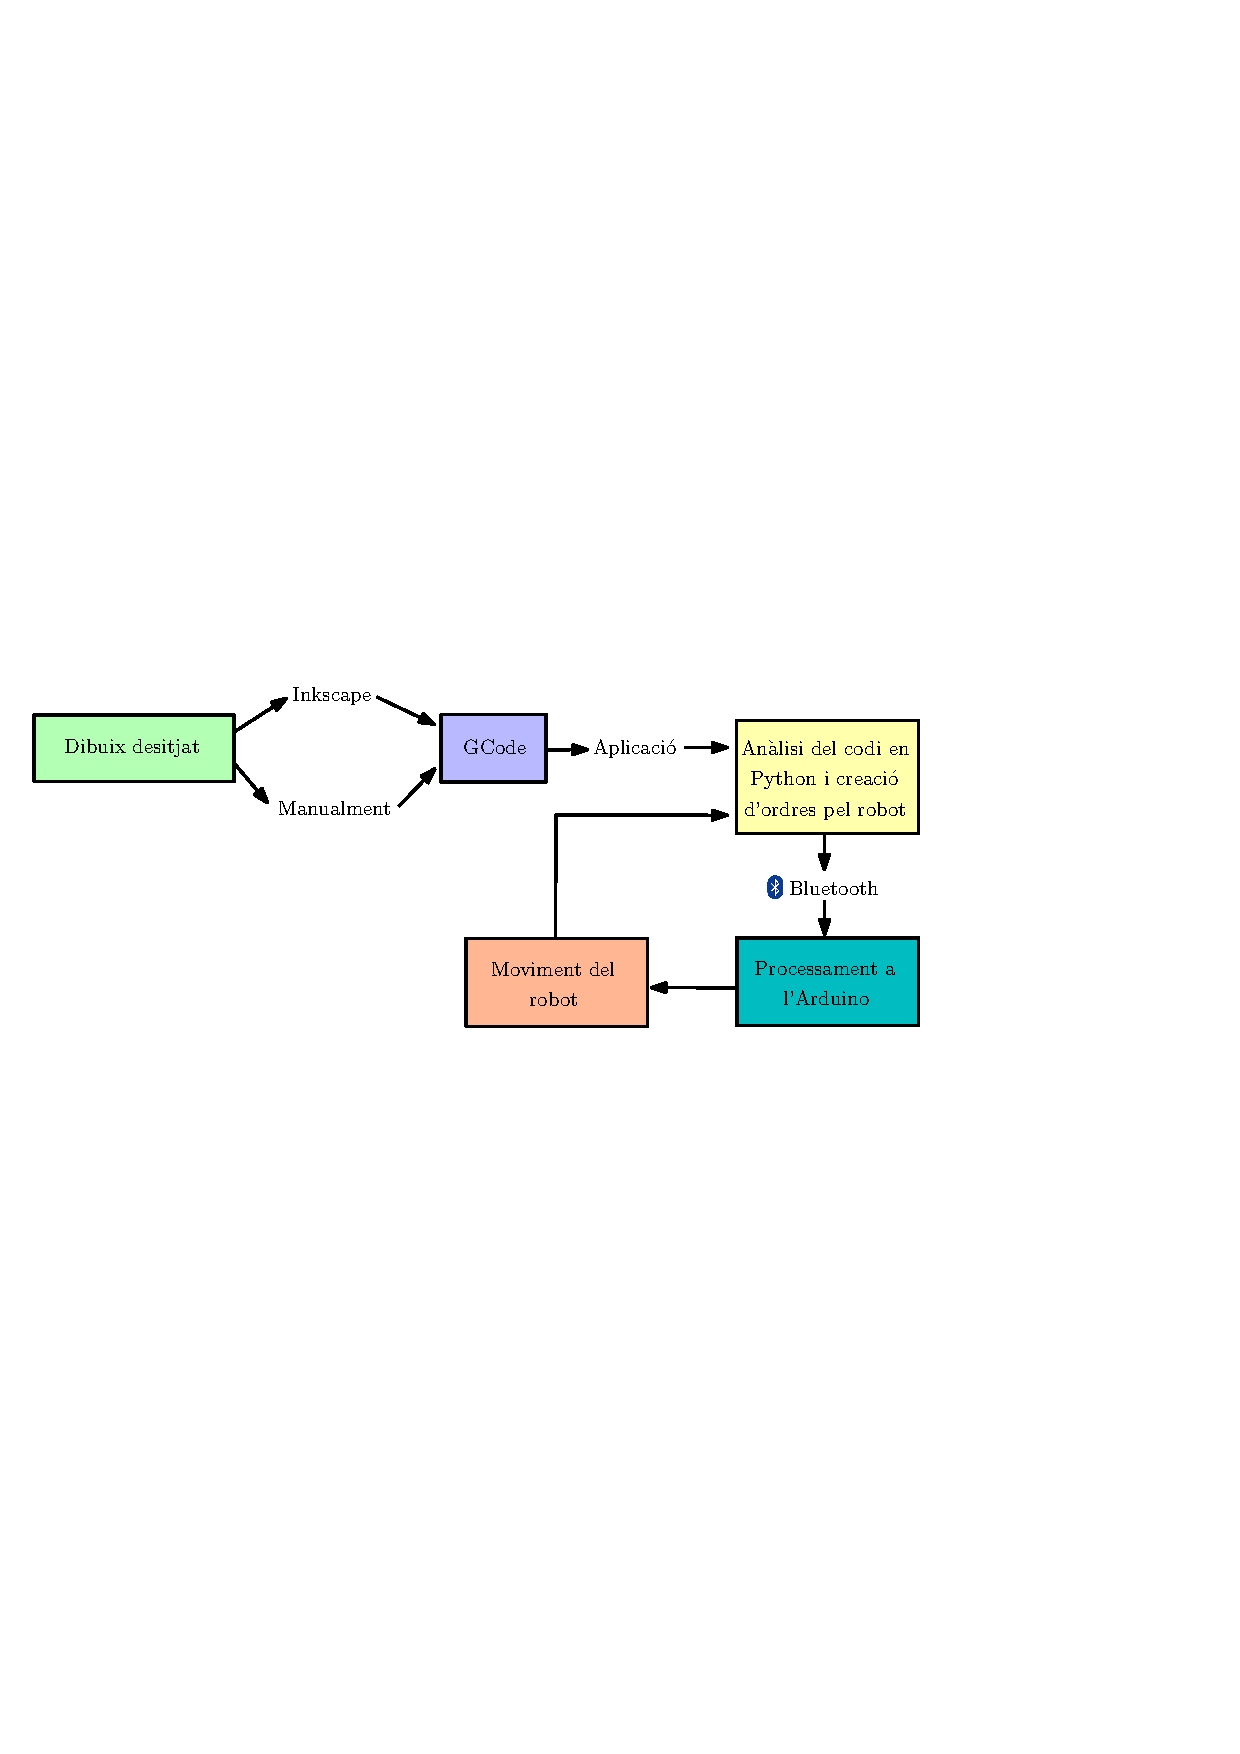
\includegraphics{figuretry}
	\caption{Diagrama de flux del procés.}
	\label{fig:diagflux}
\end{figure}




\section{GCode: Com es calcula la trajectòria?}

\subsection{Què és el GCode?}
El GCode és el llenguatge de programació més utilitzat a l'actualitat pel control de màquines CNC de control numèric com ara torns, fresadores i impressores 3D \cite{petersmid2008} . Tot i que existeixen diferents dialectes del mateix codi, tots segueixen unes normes bàsiques que el fan entenedor. La seva funció és descriure el comportament de la màquina, “què” farà i “com” ho farà, controlant la trajectòria, les velocitats de tall i avanç i el posicionament de l'eina, entre d'altres.

L'estructura del llenguatge és molt simple: cada línia de codi representa una nova instrucció o bloc i, per tant, es llegeix per línies. Hi ha diferents tipus d'ordres i per diferenciar-les es segueix una combinació de lletres i números. Sempre segueix la mateixa estructura, cada ordre es representa com una lletra seguida d'un número i dins una mateixa línia es poden combinar més d'una ordre. La lletra diferencia entre els diferents tipus comandes, per exemple, la lletra “G” s'utilitza per comandes de moviments, la “M” per comandes miscel·lànies auxiliars o de configuració i “X”, “Y” i “Z” com a posició absoluta o incremental del punts d'aplicació.  

\subsection{Comandes principals}
Les comandes més utilitzades, i les que s'utilitzaran principalment en el treball, són:

\begin{itemize}
	\item	G00: Posicionament ràpid. Comanda que, acompanyada amb la posició final X, Y i Z, posiciona l'eina de forma ràpida fins a la posició indicada. De totes les comandes que es descriuen en aquest apartat, juntament amb l'ordre G01 de rotació que s'explica a continuació, són les úniques en què l'eina no treballa, només es mou. Exemple: \emph{G00 X0 Y100 Z0}.
	
	\item	G01: Moviment en línia recta. L'eina realitza un moviment rectilini fins a la posició indicada per les lletres X, Y i Z. També es pot definir la velocitat de treball amb la comanda F. En aquest cas l'eina està en posició activa i per tant el seu moviment queda representat. Exemple: \emph{G01 X100 Y100 Z0 F100}. 
	
	\item G01 de rotació: Per altra banda, la comanda G01 també s'utilitza per rotar l'eina i corregir la seva orientació. Per fer-ho s'acompanya la comanda  amb la lletra A seguida de la direcció desitjada en radians, per exemple: \emph{G01 A3.141592}.
	
	\item	G02 i G03: Arc de circumferència.  Moviment circular en sentit horari (G02) o antihorari (G03) fins a les coordenades de destí definides com X, Y i Z. La velocitat serà la mateixa que s'hagi definit anteriorment o bé es pot tornar a assignar amb la mateixa comanda F. El moviment es pot definir pel radi amb la comanda R o pel centre de la circumferència amb les comandes I i J, sent aquestes tres les coordenades en els eixos X, Y i Z del centre. Exemple: \emph{G02 X200 Y100 Z0 I150 J0}. Tot i que les coordenades del punt final siguin coordenades absolutes, les del centre acostumen a ser incrementals respecte el punt d'origen.
	
	\item	M3: Inici de programa. Així s'indica l'inici del programa.
	
	\item	M30: Fi del programa. Amb aquesta comanda es tanca el programa. 
\end{itemize}
Existeixen moltes més ordres, però aquestes són les principals i les que utilitza l'escriptor de codi  del programa Inkscape, que és el que es vol utilitzar en aquest cas. Aquestes comandes \emph{G} són les úniques programades per ser llegides pel robot, així que són les úniques a tenir en compte. 



\section{Inkscape: Com es crea el GCode?}

\subsection{Inkscape}

Inkscape és un editor de gràfics vectorial de codi lliure i gratuït que permet crear il·lustracions, formes, gràfics, dibuixos i molt més en format vectorial .SVG (Scalable Vector Graphics) \cite{InkTutorial}. L'avantatge que té és que crea un arxiu que conté aquesta figura de manera vectorial, i això ens ajuda a crear a partir del dibuix un codi basat en GCode que s'utilitzarà per guiar el robot i definir la seva trajectòria. Aquest codi es pot guardar com un arxiu de text \emph{.txt} i serà aquest el que utilitzarà el robot per executar el programa.

Es recomana utilitzar la versió del programa 0.91 \cite{InkBib}, ja que l'actualització 0.92 té un error amb la creació dels punts d'orientació i no es respecta l'escala desitjada. 

\begin{figure}[H]
	\centering
	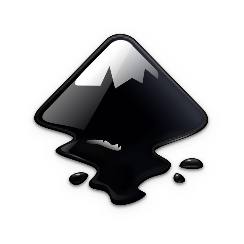
\includegraphics[scale=1]{inkscape-logo.eps}
	\caption{Logo del programa Inkscape.}
	\label{fig:inkscapelogo}
\end{figure}

\subsection{Com crear l'arxiu GCode a partir d'Inkscape} \label{sec:ManualInk}

Aquí es mostraran els passos a seguir per tal de passar un dibuix d'Inkscape a GCode amb l'extensió pròpia del programa Gcodetools.

\begin{itemize}
	
	\item	Realitzar el dibuix: El primer pas és realitzar el dibuix que es vol enviar al robot perquè aquest el dibuixi. És important definir les mides del “paper” d'Inkscape per tenir una idea de les dimensions desitjades del dibuix. Aixó es fa des de la pestanya "Archivo/Propiedades del documento”. A partir d'aquí ja es pot dibuixar el que es vulgui des del propi Inkscape. La col·locació del dibuix al full serà la desitjada per l'usuari, tenint en compte que l'origen de coordenades serà sempre l'extrem inferior esquerra. 
	
	\begin{figure}[H]
		\centering
		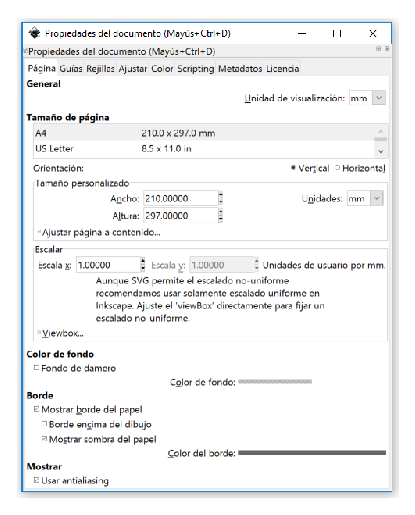
\includegraphics[scale=1.5]{1PropDocumento.eps}
		\caption{Pestanya de "Propiedades del documento".}
		\label{fig:PropDocumento}
	\end{figure}
	
	\item Convertir l'objecte en un trajecte: Amb l'objecte ja dibuixat, el següent pas és convertir-lo a una trajectòria, vectoritzar el dibuix en vectors rectes o arcs de circumferència per crear després el codi GCode de la figura. Primer cal seleccionar l'opció de “Desvío dinámico” del menú i després seleccionar al menú “Objeto” la pestanya “Objeto a trayecto”.
	
	\begin{figure}[H]
		\centering
		\includegraphics[width=0.60\linewidth]{2trayecto.eps}
		\caption{Opcions a escollir per convertir l'objecte en trajecte.}
		\label{fig:objeto a trayecto}
	\end{figure}
	
	\item Crear els punts de referència: A partir d'aquí ja es treballarà amb l'extensió Gcodetools. Fent click a l'opció “Extensiones/Gcodetools/Puntos de referencia...” es podrà veure que apareixen la referència (0,0,0) a la cantonada inferior esquerra com a origen de coordenades, que voldrà dir que s'ha creat correctament. Això indica que l'origen del dibuix, el punt on situarem el robot inicialment, serà la cantonada inferior esquerra del paper on es vulgui fer el dibuix, com s'ha explicat anteriorment.
	
	\begin{figure}[H]
		\centering
		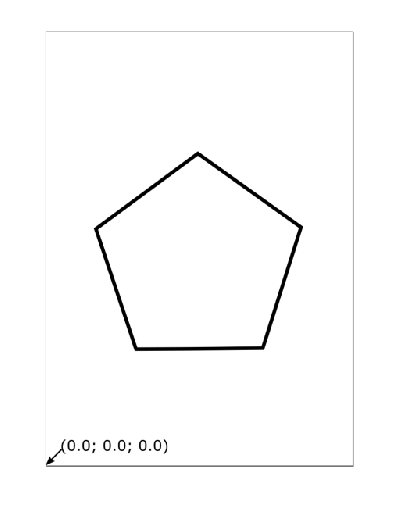
\includegraphics[width=0.40\linewidth]{3PuntosReferencia.eps}
		\caption{Punt de referència creat correctament.}
		\label{fig:PuntosReferencia}
	\end{figure}
	
	\item Seleccionar l'eina de treball: L'Inkscape té diferents eines de treball per generar el GCode i cadascuna es caracteritza per una forma diferent de treballar, fet que s'associa amb un canvi en el codi GCode. Per aquesta aplicació, l'eina més interessant i que millor s'adapta és el “Cuchillo tangencial”, que a part de la trajectòria del punter també té en compte l'orientació de l'eina, en aquest cas del robot, fet que donarà peu a un codi més fàcil de llegir pel robot, que s'estalviarà calcular aquesta orientació. Per seleccionar-la, només cal dirigir-se a la pestanya “Extensiones/Gcodetools/Biblioteca de herramientas...” y seleccionar l'opció desitjada. Un cop seleccionada s'obre un requadre verd en el que es poden modificar els paràmetres de l'eina amb l'eina d'edició de text.
	
	\begin{figure}[H]
		\centering
		\includegraphics[width=0.60\linewidth]{4tool.eps}
		\caption{Quadre de text per a la configuració de l'eina "Tangent knife".}
		\label{fig:tool}
	\end{figure}
	
	\item Crear la trajectòria de G-code: Per acabar, ja només caldrà crear l'arxiu amb el GCode. Per fer-ho, s'utilitza l'opció “Extensiones/Gcodetools/Trayecto a GCode...” on es pot modificar el nom i la direcció on es guardarà l'arxiu a la pestanya "Preferencias". Escriurem el nom de l'arxiu acabat amb l'extensió \emph{.txt} per després poder-lo llegir. Tornant a la pestanya "Trayecto a GCode", fent click a  “Aplicar” es crearà aquest arxiu y estarà llest per ser llegit amb l'Arduino.
	
	\begin{figure}[H]
		\centering
		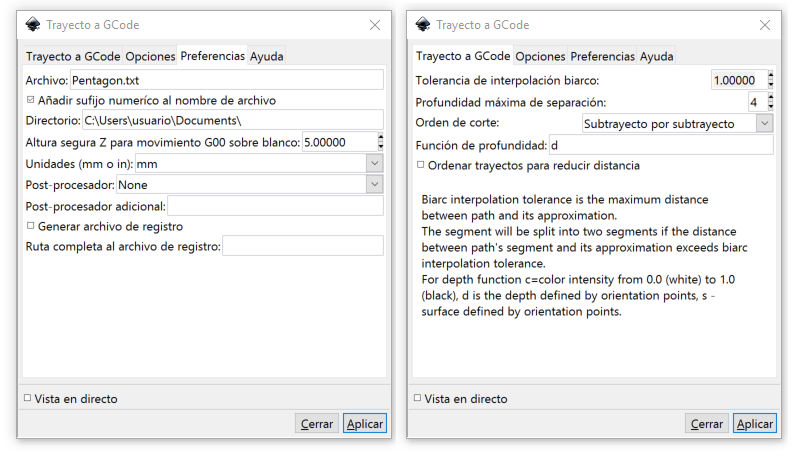
\includegraphics[width=0.60\linewidth]{5Trajectoria.eps}
		\caption{Menús necessaris per crear la trajectòria.}
		\label{fig:trayecto}
	\end{figure}
	
\end{itemize}
És important tancar les finestres sempre que acabem una operació abans de fer la següent ja que pot comportar errors. 

\section{Python: Com es processa el GCode?}

Amb el llenguatge de programació Python s’ha creat un programa capaç de llegir un arxiu .txt creat amb Inkscape i traduir-ho a moviments del robot. En aquest apartat s’explicarà què és el codi Python, el funcionament del programa principal i totes les seves funcions. 

\subsection{Introducció al Python}
El Python és un llenguatge de programació lliure (Open Source) que té com a objectiu mantenir la simplicitat i ser un codi fàcil de llegir, entendre i aprendre \cite{mariadolorsayalavallesp2016} \cite{jeffreyelknerallenb.downeyichrismeyers2012}. Al ser un codi lliure està en constant creixement ja que tothom pot aportar-hi els seus coneixements i la comunitat de programadors Python és enorme, per la qual cosa és fàcil d’apendre a partir de llibres, manuals o tutorials online. 

Aquest llenguatge és el llenguatge après a la universitat durant el grau i és per això que s’ha decidit utilitzar-lo. S’ha instal·lat la versió de Python 2.7 directament des de la seva pàgina web \cite{PythonWeb}. Als següents apartats s’explicarà el funcionament del programa i el seu codi. 

\begin{figure}[H]
	\centering
	
\includegraphics[scale=0.5]{python-logo.png}
	\caption{Logo del programa Python.}
	\label{fig:pythonlogo}
\end{figure}

\subsection{El programa}\label{sec:robotmoveBT}

El programa encarregat de moure el robot es troba dins l’arxiu “RobotMoveBT.py” que es pot trobar a l’annex \ref{PyRobot} i el seu funcionament es basa en diferents funcions. L’objectiu del programa és llegir l’arxiu GCode creat i traduir cadascuna de les ordres en passos del motor i la posició del servo per tal d’enviar-ho després a l’Arduino. 

En primer lloc, a l'executar l’arxiu s’importen diferents llibreries: la llibreria “math” que ens permet fer operacions matemàtiques complexes, “serial” per tal de comunicar l’ordinador i l’Arduino i “time” per tal de programar temps d’espera per una bona comunicació. Tot seguit s’inicia la comunicació amb el Robot mitjançant la següent comanda:

\begin{python}
	import math, serial, time
	arduino=serial.Serial('COM4', 9600)
\end{python}

Cal notar que el port ‘COM4’ és el port que ocupa la connexió Bluetooth i que, per tant s’ha de configurar abans d’executar-lo si s’utilitza des d’un altre ordinador. 

A partir d’aquí es defineixen una sèrie de variables globals que serviran per tot el programa, les quals s’utilitzaran en les altres funcions. Defineixen els paràmetres bàsics del Robot i la seva configuració. 

\begin{python}
	StepsVolta=1600  #passos per realitzar una volta completa del motor
	x0 = 0.0  #coordenades absolutes que ocupa el robot
	y0 = 0.0  #coordenades absolutes que ocupa el robot
	pasdreta=0  #posicio absoluta del motor dret en pasos
	pasesquerra=0  #posicio absoluta del motor dret en pasos
	DiamRoda=51.9  #diametre de la roda en mm
	RadiRoda=DiamRoda/2.0  #radi de la roda en mm
	distDreta=61.8  #distancia en mm entre el centre de l'eix (punt del boli) i la roda dreta
	distEsquerra=61.9  #distancia en mm entre el centre de l'eix (punt del boli) i la roda esquerra
	pas= math.pi *DiamRoda/StepsVolta  #mm recorreguts per pas del motor
	direccio0=math.pi/2  #angle inicial del robot a 90 graus
	tempsLectura=0.01  #temps per llegir l'Arduino 
\end{python}


Un cop definides les variables inicials s’han creat diferents funcions que es poden separar en dos grans apartats: funcions de moviment del robot i funcions de lectura. 

\subsection{Funcions de moviment del robot}
S’han definit les funcions bàsiques per tal d’actuar amb les diferents comandes de GCode que poden aparèixer, G00, G01, G02, G03 i G01 de rotació. L’objectiu d’aquestes és calcular els passos que ha de realitzar cada motor per tal de seguir el moviment definit. 

\subsubsection{Funció G00($x_{1}$, $y_{1}$)}\label{sec:G00}

Aquesta funció realitza un moviment rectilini fins al punt definit per les coordenades d’entrada ($x_{1}$,$y_{1}$) amb el retolador aixecat, de tal manera que aquest moviment no quedarà representat en el dibuix final, és un moviment de posicionament.

\begin{figure}[H]
	\centering
	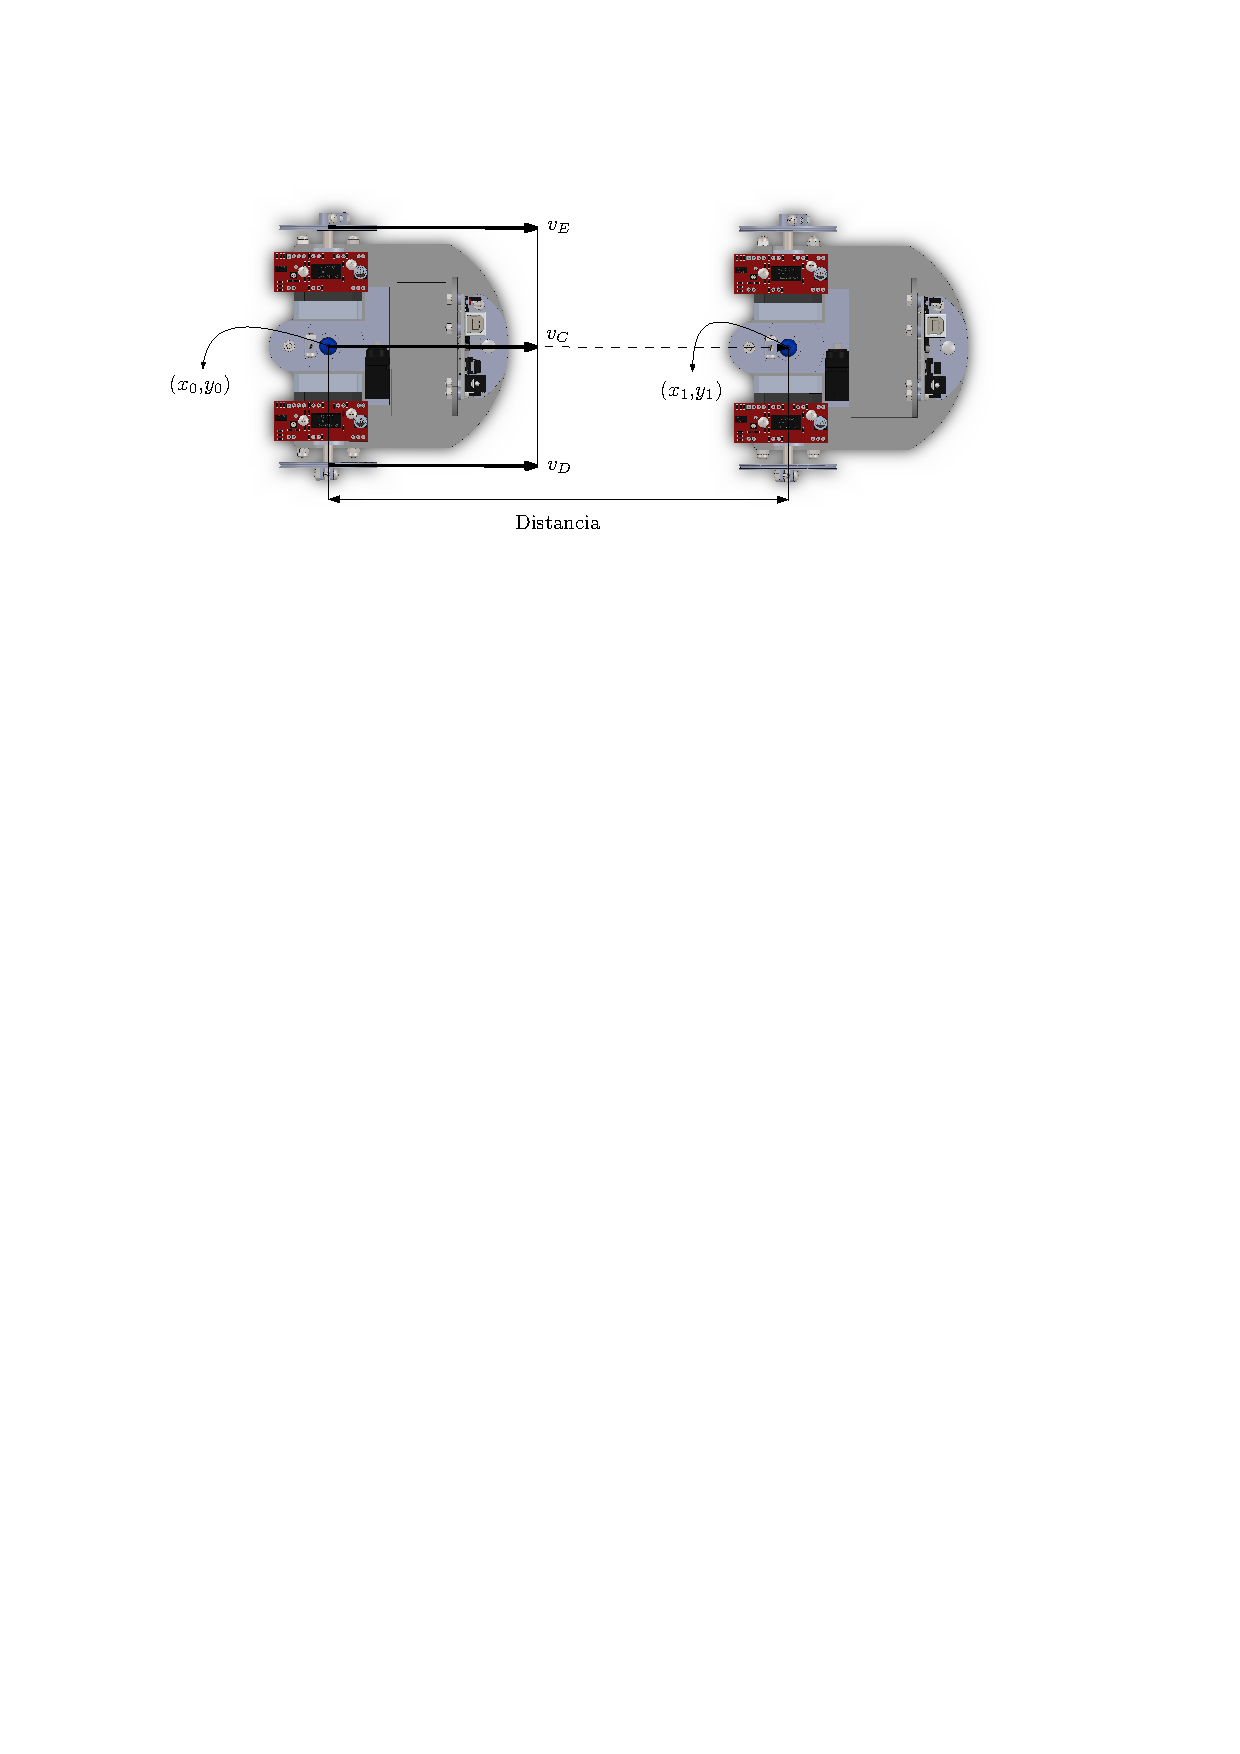
\includegraphics[scale=0.9]{G00}
	\caption{Representació d'un moviment amb l'ordre G00.}
	\label{fig:G00}
\end{figure}


En el cas de l’ordre G00, el primer que cal fer és rotar el robot per tal de posicionar-lo en direcció al punt de destí ($x_{1}$, $y_{1}$). És en l'única operació que cal fer-ho, ja que, a l'utilitzar l’eina “Cuchillo tangencial” d’Inkscape , sempre que hi ha un moviment amb el retolador en posició activa primer es realitza una ordre G01 A\emph{X} que rota el robot fins a la direcció (\emph{X}) adequada per començar el moviment. En aquest cas, al tenir el retolador aixecat el propi Inkscape entén que es pot moure fins a les coordenades destí de qualsevol manera, però com que el moviment del robot és empre en una única direcció, cal rotar-lo per tal d'apuntar cap al punt final i realitzar un moviment rectilini. Aquest càlcul es fa utilitzant l’arctangent del valor de $\frac{\Delta y }{\Delta x}$ amb el següent codi:
\begin{python}
	if (dx != 0):
		direccio = math.atan(dy/dx) 
	if (dx < 0 and dy >= 0):
		direccio = direccio + math.pi 
	elif (dx < 0 and dy < 0):
		direccio = direccio - math.pi
		apuntar(direccio) 
	else:
		if (dy > 0):
			direccio = math.pi/2.0 
		elif (dy<0):
			direccio = -math.pi/2.0 
		else:
			direccio=direccio0
		apuntar(direccio) 
	direccio0=direccio
\end{python}

Com es pot observar, si la direcció és vertical $(\pm\frac{\pi}{2})$  l’arctangent és infinit i no es pot calcular, per això s’estudia apart. Per altra banda, si l’angle pertany al segon i tercer quadrant, cal sumar i restar pi respectivament per aconseguir l’angle desitjat, ja que els angles resultants de l’operació arctangent estan compresos sempre a l’interval $[-\frac{\pi}{2}, \frac{\pi}{2}]$.

Per calcular els passos que ha de fer el motor només cal calcular la distància que hi ha entre el punt inicial i el final i, dividint aquesta distància pel nombre de mil·límetres recorreguts per cada pas de la roda, s’obté el nombre de passos a realitzar arrodonit a l'enter més proper. 

\begin{equation}\label{eq:dist}
Dist\grave{a}ncia=\sqrt{\Delta x^2+ \Delta y^2}
\end{equation}

\begin{equation}\label{eq:pas}
Pas=\frac{\pi\cdot Di\grave{a}metre \ de \ la \ roda}{Steps/volta}
\end{equation}

\begin{equation}\label{eq:steps}
Steps=\frac{Dist\grave{a}ncia}{Pas}
\end{equation}


Un cop acabats els càlculs es corregeixen els valors de la posició actual $(x_{0},y_{0})$, el de la direcció del robot $(direccio_{0})$ i la posició absoluta dels motors, expressada en passos del motor, que s’enviarà a l'Arduino. 

Per acabar s’estableix la connexió amb l’Arduino. En primer lloc, s’envia una cadena de valors amb el següent format: \emph{“posició del servomotor, passos del motor dret, passos del motor esquerra,”}. El primer valor indicarà la posició del servomotor, que pot ser \emph{0} si el retolador està aixecat o \emph{1} si està actiu, tocant el paper. En aquest cas sempre serà \emph{0}. Els dos valors següents són les posicions absolutes dels motors expresades en passos del motor. Cal acabar la cadena amb una coma \emph{“,”} ja que és així com s’ha programat l’Arduino. Un cop enviada, el programa entra en un bucle que el manté inactiu fins que rep de l’Arduino la paraula \emph{“Ready”}, senyal que ja es pot enviar una nova ordre. Aixó s’aconsegueix mitjançant el següent codi:

\begin{python}
	text='0'+','+str(pasdreta)+','+str(pasesquerra)+','
	arduino.write(text)
	robot=1
	while robot==1:
		if arduino.inWaiting()>0:
			st=arduino.readline().strip()
			time.sleep(tempsLectura)
			if st=='Ready':
				robot=0
\end{python}

\subsubsection{Funció G01($x_{1}$, $y_{1}$)}
El funcionament d’aquesta funció és exactament igual a la funció G00, ja que també és un moviment rectilini, però aquest cop el retolador sí que ha de traçar una línia. L'única diferència entre aquestes és que en el cas de l’ordre G01 no cal redireccionar el robot per apuntar al punt de destí, perquè el propi Inkscape crearà prèviament una ordre espeífica per fer-ho que s’explicarà a l’apartat \ref{apuntar}. Per altra banda, en aquest cas, el primer valor que s’envia a l’Arduino serà un \emph{1} ja que la posició del servo ha de ser posició activa amb la qual el retolador està dibuixant. 

\begin{figure}[H]
	\centering
	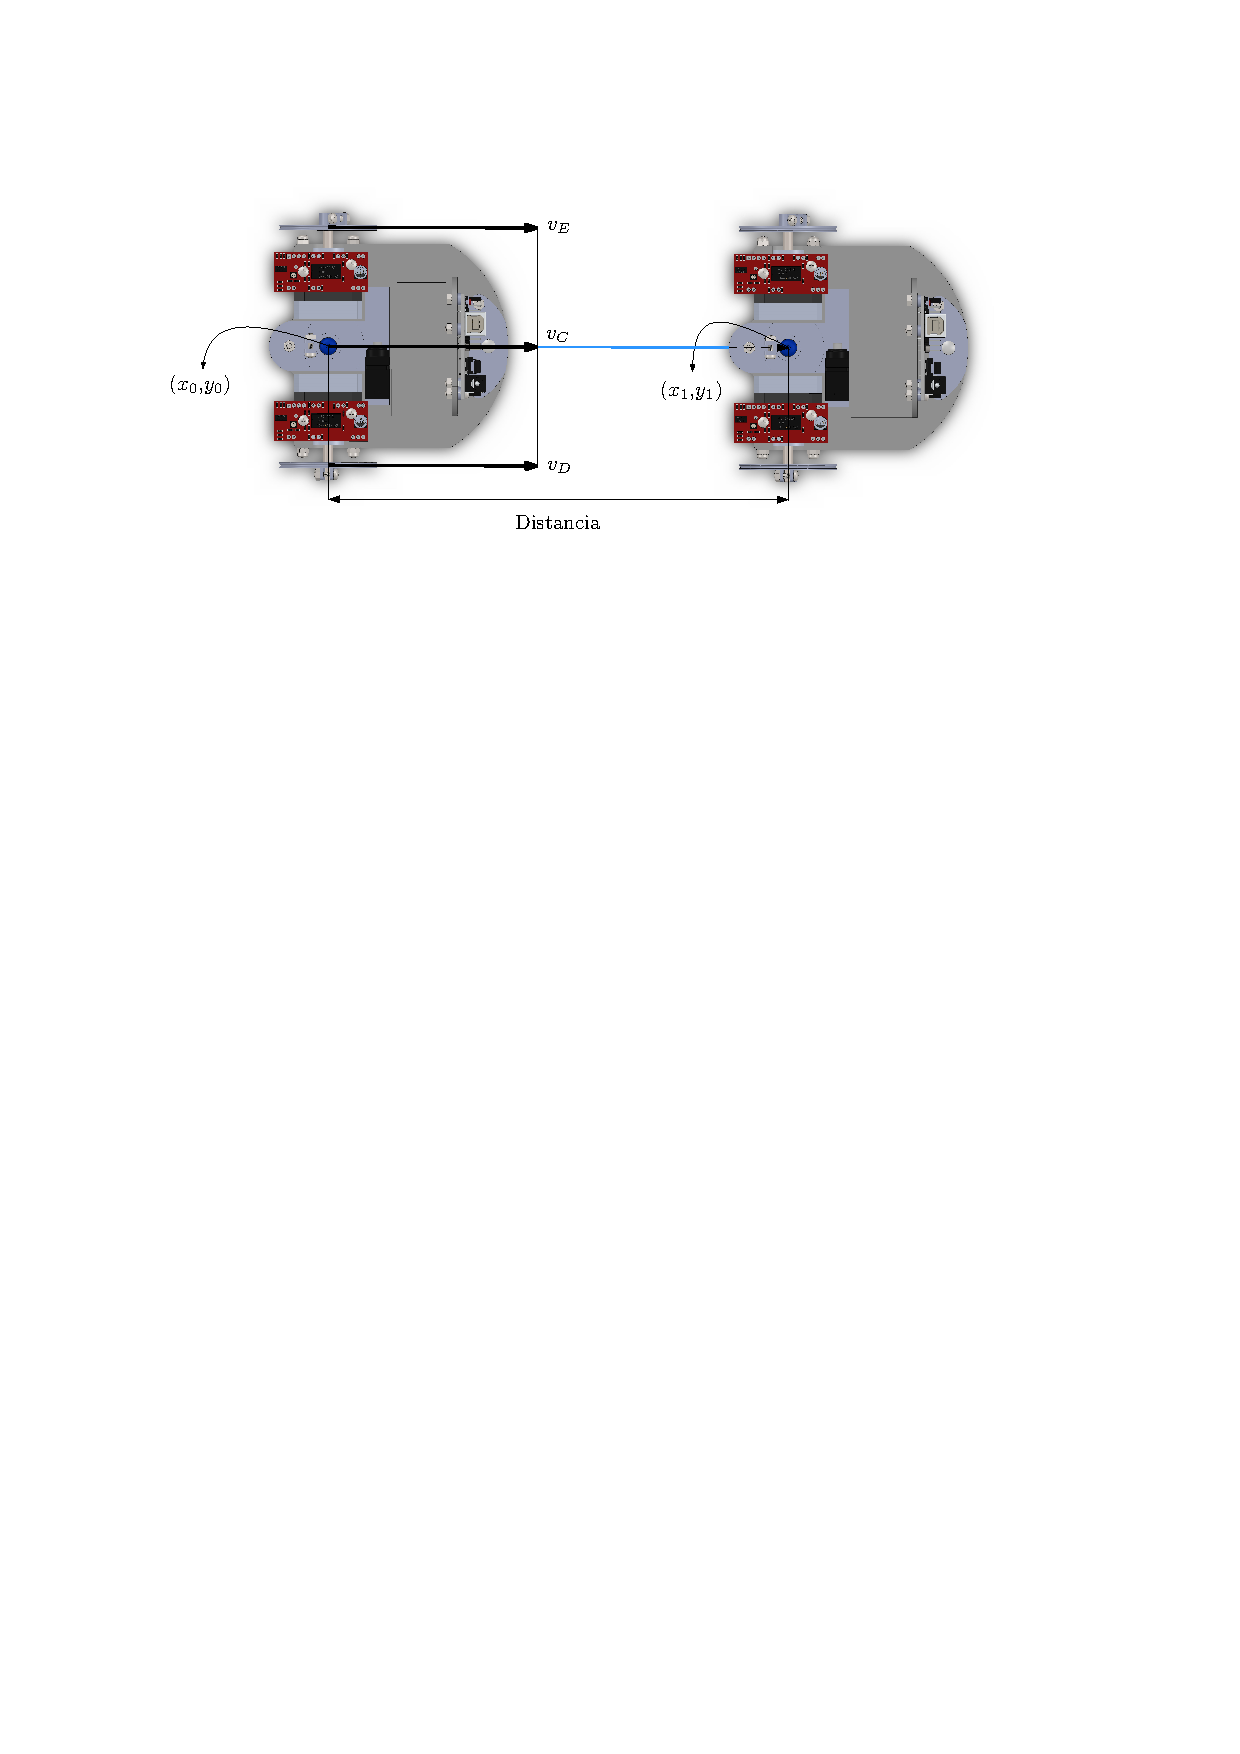
\includegraphics[scale=0.9]{G01}
	\caption{Representació d'un moviment amb l'ordre G01.}
	\label{fig:G01}
\end{figure}

A diferència del G00, es pot veure a la imatge \ref{fig:G01} que amb la comanda G01 sí que es dibuixa sobre el paper (línia blava).

\subsubsection{Funció G02($x_{1}$, $y_{1}$, $x_{C}$, $y_{C}$, $direccio_{1}$)}\label{funG02}

Aquesta funció té l’objectiu de dibuixar un arc de circumferència en sentit horari. Les entrades de la mateixa són les coordenades absolutes del punt de destí ($x_{1}$, $y_{1}$), les coordenades relatives del centre de gir ($x_{C}$, $y_{C}$) respecte el punt inicial i la direcció amb la qual acabarà el moviment ($direccio_{1}$). A la figura \ref{fig:G02} es representa el moviment:

\begin{figure}[H]
	\centering
	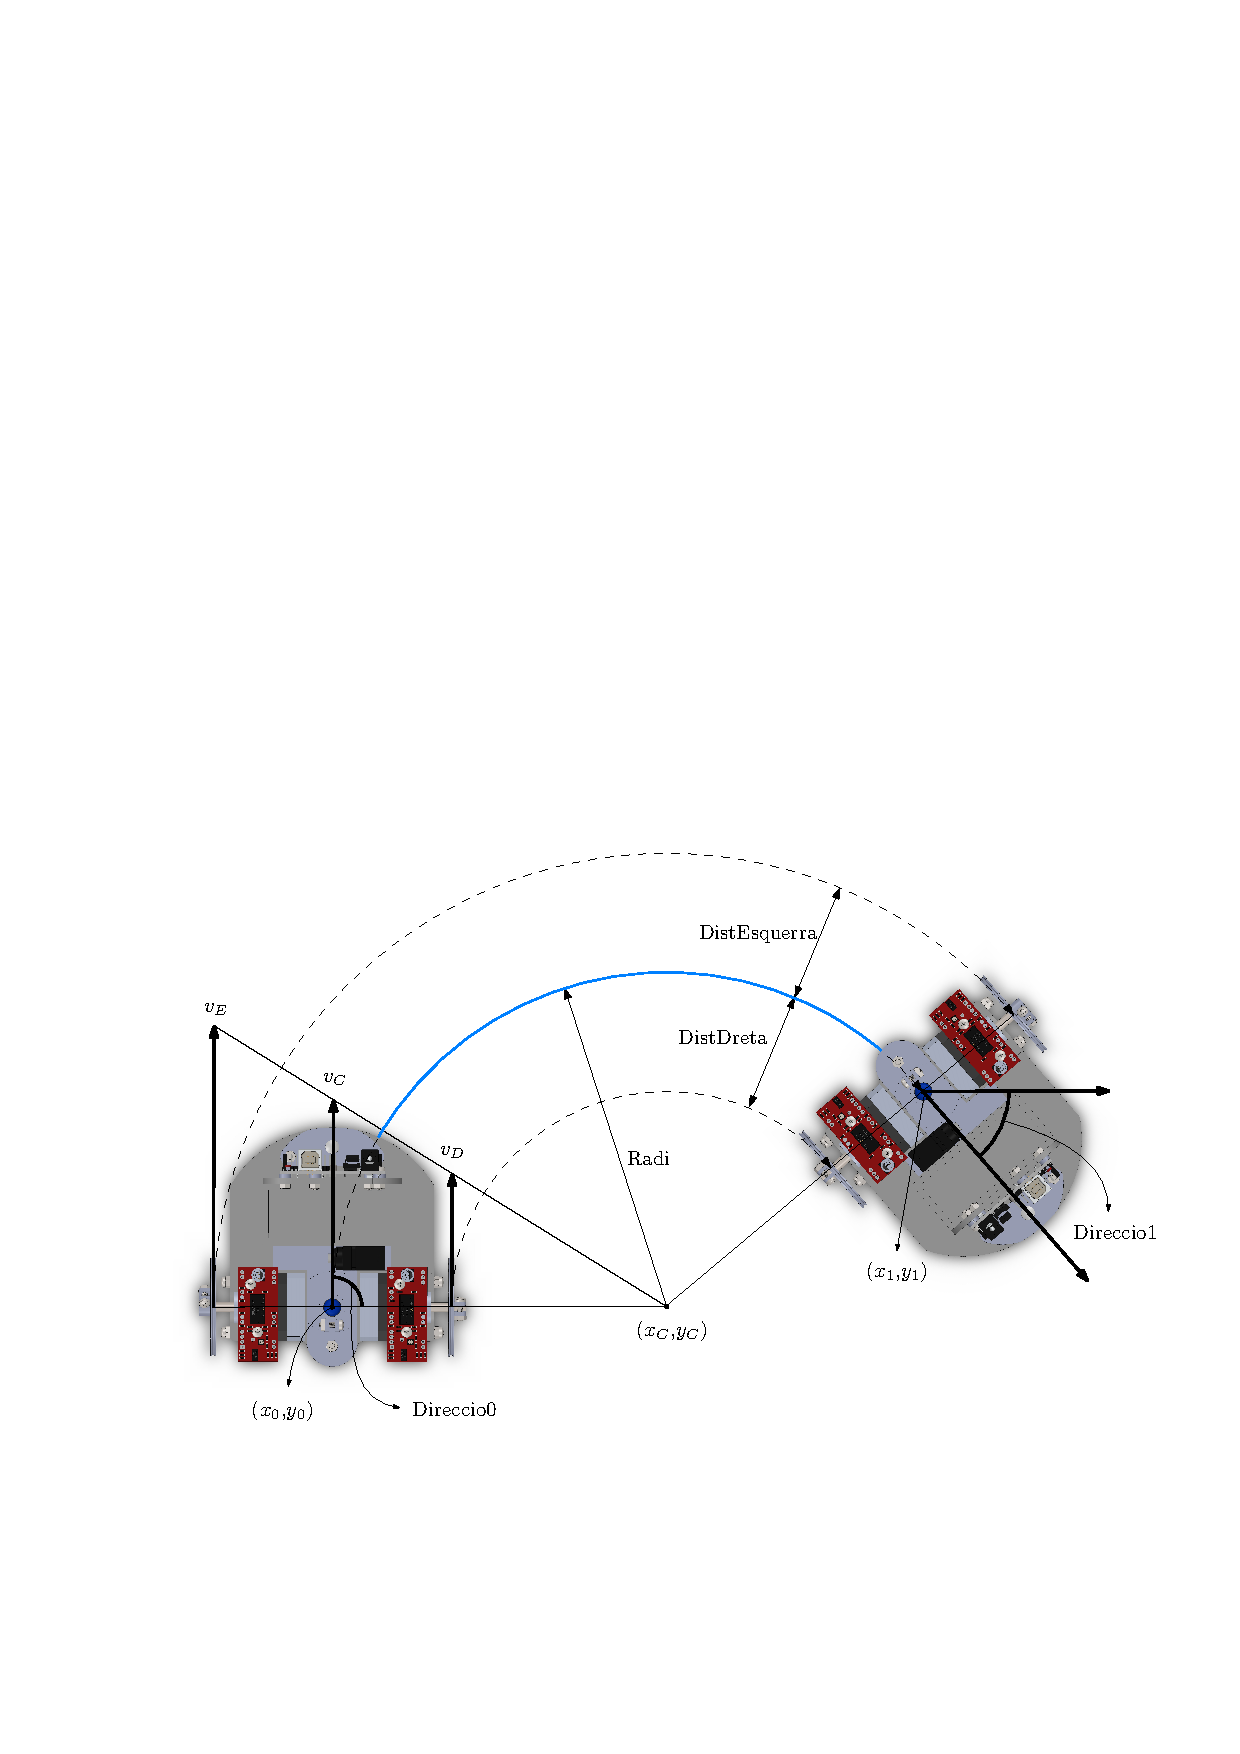
\includegraphics[scale=0.9]{G02}
	\caption{Representació d'un moviment amb l'ordre G02.}
	\label{fig:G02}
\end{figure}

Per tal de calcular els passos necessaris de cada motor per realitzar el moviment, primer es calcularà el radi de gir, aprofitant que es coneix la posició relativa, del centre de la següent manera:
\begin{equation}
Radi \ de \ gir = \sqrt{x_{C}^2+y_{C}^2}
\end{equation}


Després es realitza un canvi de coordenades per tal de definir les coordenades del centre en el punt \emph{(0,0)} de la següent manera:

Primer es calculen les coordenades absolutes del centre:
\begin{eqnarray}
\nonumber & x_{C}=x_{C}+x_{0} \\
& y_{C}=y_{C}+y_{0}
\end{eqnarray}

I després es fa el canvi de coordenades:
\begin{eqnarray}
\nonumber & x_{0}=x_{0}-x_{C} \\
\nonumber & y_{0}=y_{0}-y_{C} \\
\nonumber & x_{1}=x_{1}-x_{C} \\
& y_{1}=y_{1}-y_{C}
\end{eqnarray}

Amb les noves coordenades el primer pas és calcular l’angle de circumferència que separa els dos punts, ja que, com que el retolador està alineat amb les rodes, els tres punts de contacte posterior del robot (rodes i retolador) traçaran la mateixa trajectòria amb un radi diferent, i per tant aquest angle serà el mateix. Aquest es calcula amb les següents línies de codi:

\begin{python}
	angle0=math.atan2(y0,x0)
	angle1=math.atan2(y1,x1)
	angle=angle0-angle1
	if angle<0:
		angle=2*math.pi+angle
\end{python}

La funció \emph{math.atan2(y,x)} retorna la direcció d’aquest punt, i, restant les direccions del punt inicial i el punt final, es pot calcular l'angle entre ells. Si l’angle resultant és menor a \emph{0} es converteix al seu respectiu angle en positiu, sumant $2\pi$, per mantenir-se sempre a l’interval $[\emph{0},\emph{2} \pi]$.

Un cop calculat l’angle, s’utilitzen les següents equacions per calcular la distància que han de recórrer cadascuna de les rodes tenint en compte la variació de radi:
\begin{eqnarray}
\nonumber &Dist. \ recorregut \ R.D. = Angle \cdot (Radi \ de \ gir-Dist. \ R.D. \ a \ C) \\ 
&Dist. \ recorregut \ R.E. = Angle \cdot (Radi \ de \ gir-Dist. \ R.E. \ a \ C)
\end{eqnarray}
Essent  $(Dist. \ R.D. \ a \ C)$ i $(Dist. \ R.E. \ a \ C)$ les distàncies entre les rodes (\emph{R.D.} dreta o \emph{R.E.} esquerra) fins al centre (C).

Amb el valor de les distàncies i utilitzant l’equació (\ref{eq:steps}) es calculen els passos a recórrer per cada motor, s’actualitzen les dades i s’envia la comanda a l’Arduino de la mateix manera que s’ha explicat amb la funció G00, però amb la posició del servo igual a \emph{1} ja que el retolador ha d’estar actiu. 

\subsubsection{Funció G03($x_{1}$, $y_{1}$, $x_{C}$, $y_{C}$, $direccio_{1}$)}
El funcionament és exactament igual al G02, però en aquest cas el gir serà en sentit antihorari. L'única diferència es troba en el càlcul de l’angle i en la variació del radi de gir, que es canvien en el codi de la següent manera: \\


\begin{python}
	angle=angle1-angle0
	...
	distanciaD = angle * (RadiGirC+distDreat) 
	distanciaE = angle * (RadiGirC-distEsquerra)
\end{python}
\subsubsection{Funció apuntar($direccio_{1}$)}\label{apuntar}

Aquesta és la funció encarregada de la rotació del robot. S’utilitza quan l’ordre del GCode és G01 A\emph{X} on \emph{X} és la direcció a la qual ha d’apuntar el robot i dins la funció G00 per tal de redireccinar-lo. 

El càlcul de passos consisteix, en primer lloc, en la decisió del sentit de gir per tal de saber quin és el camí més curt, que es troba amb les següents línies de codi:
\begin{python}
	gir=direccio0-direccio1 
	absgir=abs(gir) 
	if (absgir > math.pi):
		if (gir<0):
			gir= 2.0 * math.pi + gir 
		else:
			gir= -2.0 * math.pi + gir
\end{python}
Si el valor de la variable \emph{gir}, que és l’angle a girar pel robot, és negatiu girarà en sentit antihorari, i sinó en sentit horari. Aquest angle mai serà superior a $\pi$. 

En segon lloc cal calcular els passos dels motors. Aquest càlcul es basa en l’equació (\ref{eq:steps}) de l’apartat G00. En aquest cas, el valor de la posició del servo és \emph{0}, ja que s’ha decidit així per tal de no mantenir el contacte del retolador amb el paper i evitar taques de tinta als punts de gir. 





\section{Arduino: Qui mou el robot?}

Arduino es presenta com una plataforma de codi lliure (Open Source) basat en un hardware i un software de fàcil utilització i accessible per tothom.  Permet crear prototips a partir de la lectura d’entrades (inputs) com podrien ser, per exemple, un sensor de temperatura, l’acció d’un polsador o una comunicació des de l’ordinador, i convertir-ho en una acció de sortida (output) com podria ser el moviment d’un motor, enviar un missatge a un ordinador o qualsevol dispositiu que l’usuari pugui programar. La programació de la placa es realitza mitjançant el software (IDE) lliure de la marca basat en Processing i en el seu propi llenguatge de programació Arduino basat en Wiring \cite{arduinoBib} \cite{massimobanzi2011}. 

Arduino neix a la ciutat piemontesa d’Ivrea al nord d’Itàlia al lvrea Interaction Design Institute com un projecte pels estudiants de l’institut de mans del professor Massimo Banzi. Va començar com una eina de prototipatge ràpid utilitzada per a la introducció a l’electrònica i la programació dels estudiants sense experiència. Tot i aixó, el projecte va ser molt ben acollit per la comunitat internacional convertint-se així en una eina molt utilitzada arreu del món per principiants i experts. Al llarg dels anys ha evolucionat molt per tal de brindar noves opcions als usuaris, per exemple, va realitzar una col·laboració amb Google per aconseguir comunicar directament la placa amb el sistema operatiu Android o l’adaptació de noves plaques per treballar amb aplicacions d’IoT (Internet of things) o Wearables. Totes les plaques de la companyia són Open Source igual que el software que es manté en constant creixement gràcies a l’aportació dels usuaris. 

\begin{figure}[H]
	\centering
	
\includegraphics[scale=0.1]{arduino-logo.png}
	\caption{Logo d'Arduino.}
	\label{fig:arduinologo}
\end{figure}

\subsection{Arduino UNO}

Per aquest projecte s’ha utilitzat el model Arduino UNO. Aquest model  es basa en un microcontrolador ATmega328P amb memòria flash de 32 Kb programable des del software Arduino. Presenta 14 pins digitals d’entrada/sortida, 6 dels quals es poden programar com a sortida amb modulació de pols PWM, i 6 entrades analògiques disponibles per l’usuari, un oscil·lador de quars de 16MHz, una connexió USB per connectar-lo a l’ordinador, connexió ICSP-6 per programar-la, una entrada de corrent de 5V i un polsador de reinici. 

És una placa bàsica, la primera que va sortir al mercat, ideal per a projectes petits i la iniciació en el món Arduino.

\begin{figure}[H]
	\centering
	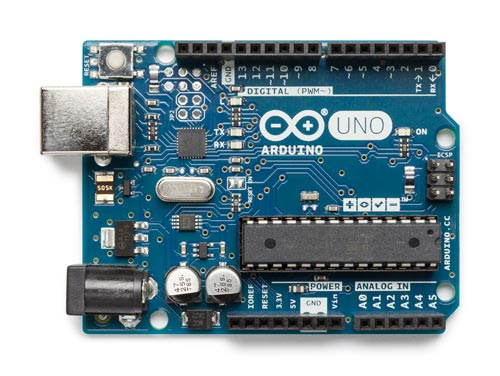
\includegraphics[scale=0.5]{arduino-uno.png}
	\caption{Placa Arduino UNO.}
	\label{fig:arduinouno}
\end{figure}

\subsection{Connexió}\label{sec:connexio}

La connexió de l’Arduino és molt important, ja que es on és connecten tots els elements del robot i l’encarregada de que tot funcioni. Seguidament es presentarà la connexió dels diferents elements.

En primer lloc, els motors es connecten a partir dels drivers i ocupen 4 entrades de la placa cadascun. Les dues primeres són els pins de STEP i Direcció del controlador, els encarregats de definir la quantitat i la direcció dels passos del motor, que es connecten als pins digitals 8 i 9 (direcció i STEP) en el cas del motor dret i 12 i 13 (direcció i STEP) en el cas del motor esquerre. Els altres dos pins que ocupen cada motor a l’Arduino són els anomenats MS1 i MS2 que, com s’ha explicat a l’apartat explicatiu del driver \ref{sec:driver}, s’encarreguen de controlar el microstepping (reduir l’angle de pas i, per tant, augmentar el nombre de passos). Aquests s’han connectat als pins digitals 2 i 3 per la roda dreta i 4 i 5 per l’esquerra. S’ha programat de manera que la sortida estigui activa (HIGH) i per tant rebi 5V, la qual cosa es traduirà en un augment de 8 vegades els passos inicials (200 passos per volta) fins 1600 passos per volta. Aquesta configuració permet augmentar considerablement la precisió de la traçada. Els pins de GND de referència dels drivers s’han connectat a les entrades GND de l’Arduino per assegurar un mateix connector a terra per tot el disseny. Per acabar, els pins d’alimentació (5V i GND) s’han connectat directament a la sortida de la font amb les dues fileres de pins de la protoboard. 

Per altra banda, el senyal de control del servomotor es connecta al pin 6 amb sortida PWM de la placa per tal de definir la posició de l’eix en funció del pols de l’entrada. Els cables de voltatge es connecten directament a les tires de pins de la protoboard a la sortida de la bateria compartida amb el motor esquerra.  S’evita així connectar-ho a la sortida de 5V de l’Arduino per repartir el consum entre les dues fonts, com ja s’ha explicat a l’apartat de la bateria \ref{sec:bateria}. 

Per acabar, es connecta el mòdul HC-05. Els senyals TX i RX, que es detallaran més endavant, actuen sobre les entrades digitals 10 i 11 respectivament, mentre que les entrades de corrent es connecten a les sortides de 3,3V i GND de l’Arduino. 

Un cop fetes totes les connexions amb els diferents components, s’alimenta l’Arduino directament des de la font compartida amb el motor dret utilitzant les entrades Vin i GND de la pròpia placa. 

Per tal de reprogramar el microcontrolador des de l’ordinador, es pot utilitzar l’entrada del port serial USB. És per aquesta raó que el mòdul Bluetooth es connecta als pins 10 i 11 i no als pins 0 i 1, reservats pels canals de lectura i escriptura. Si es connectés aquí s’hauria de desconnectar cada cop que es volgués carregar un programa a la placa, ja que es podrien crear interferències a l'estar accedint al mateix canal per dues bandes diferents alhora. 
\begin{figure}[H]
	\centering
	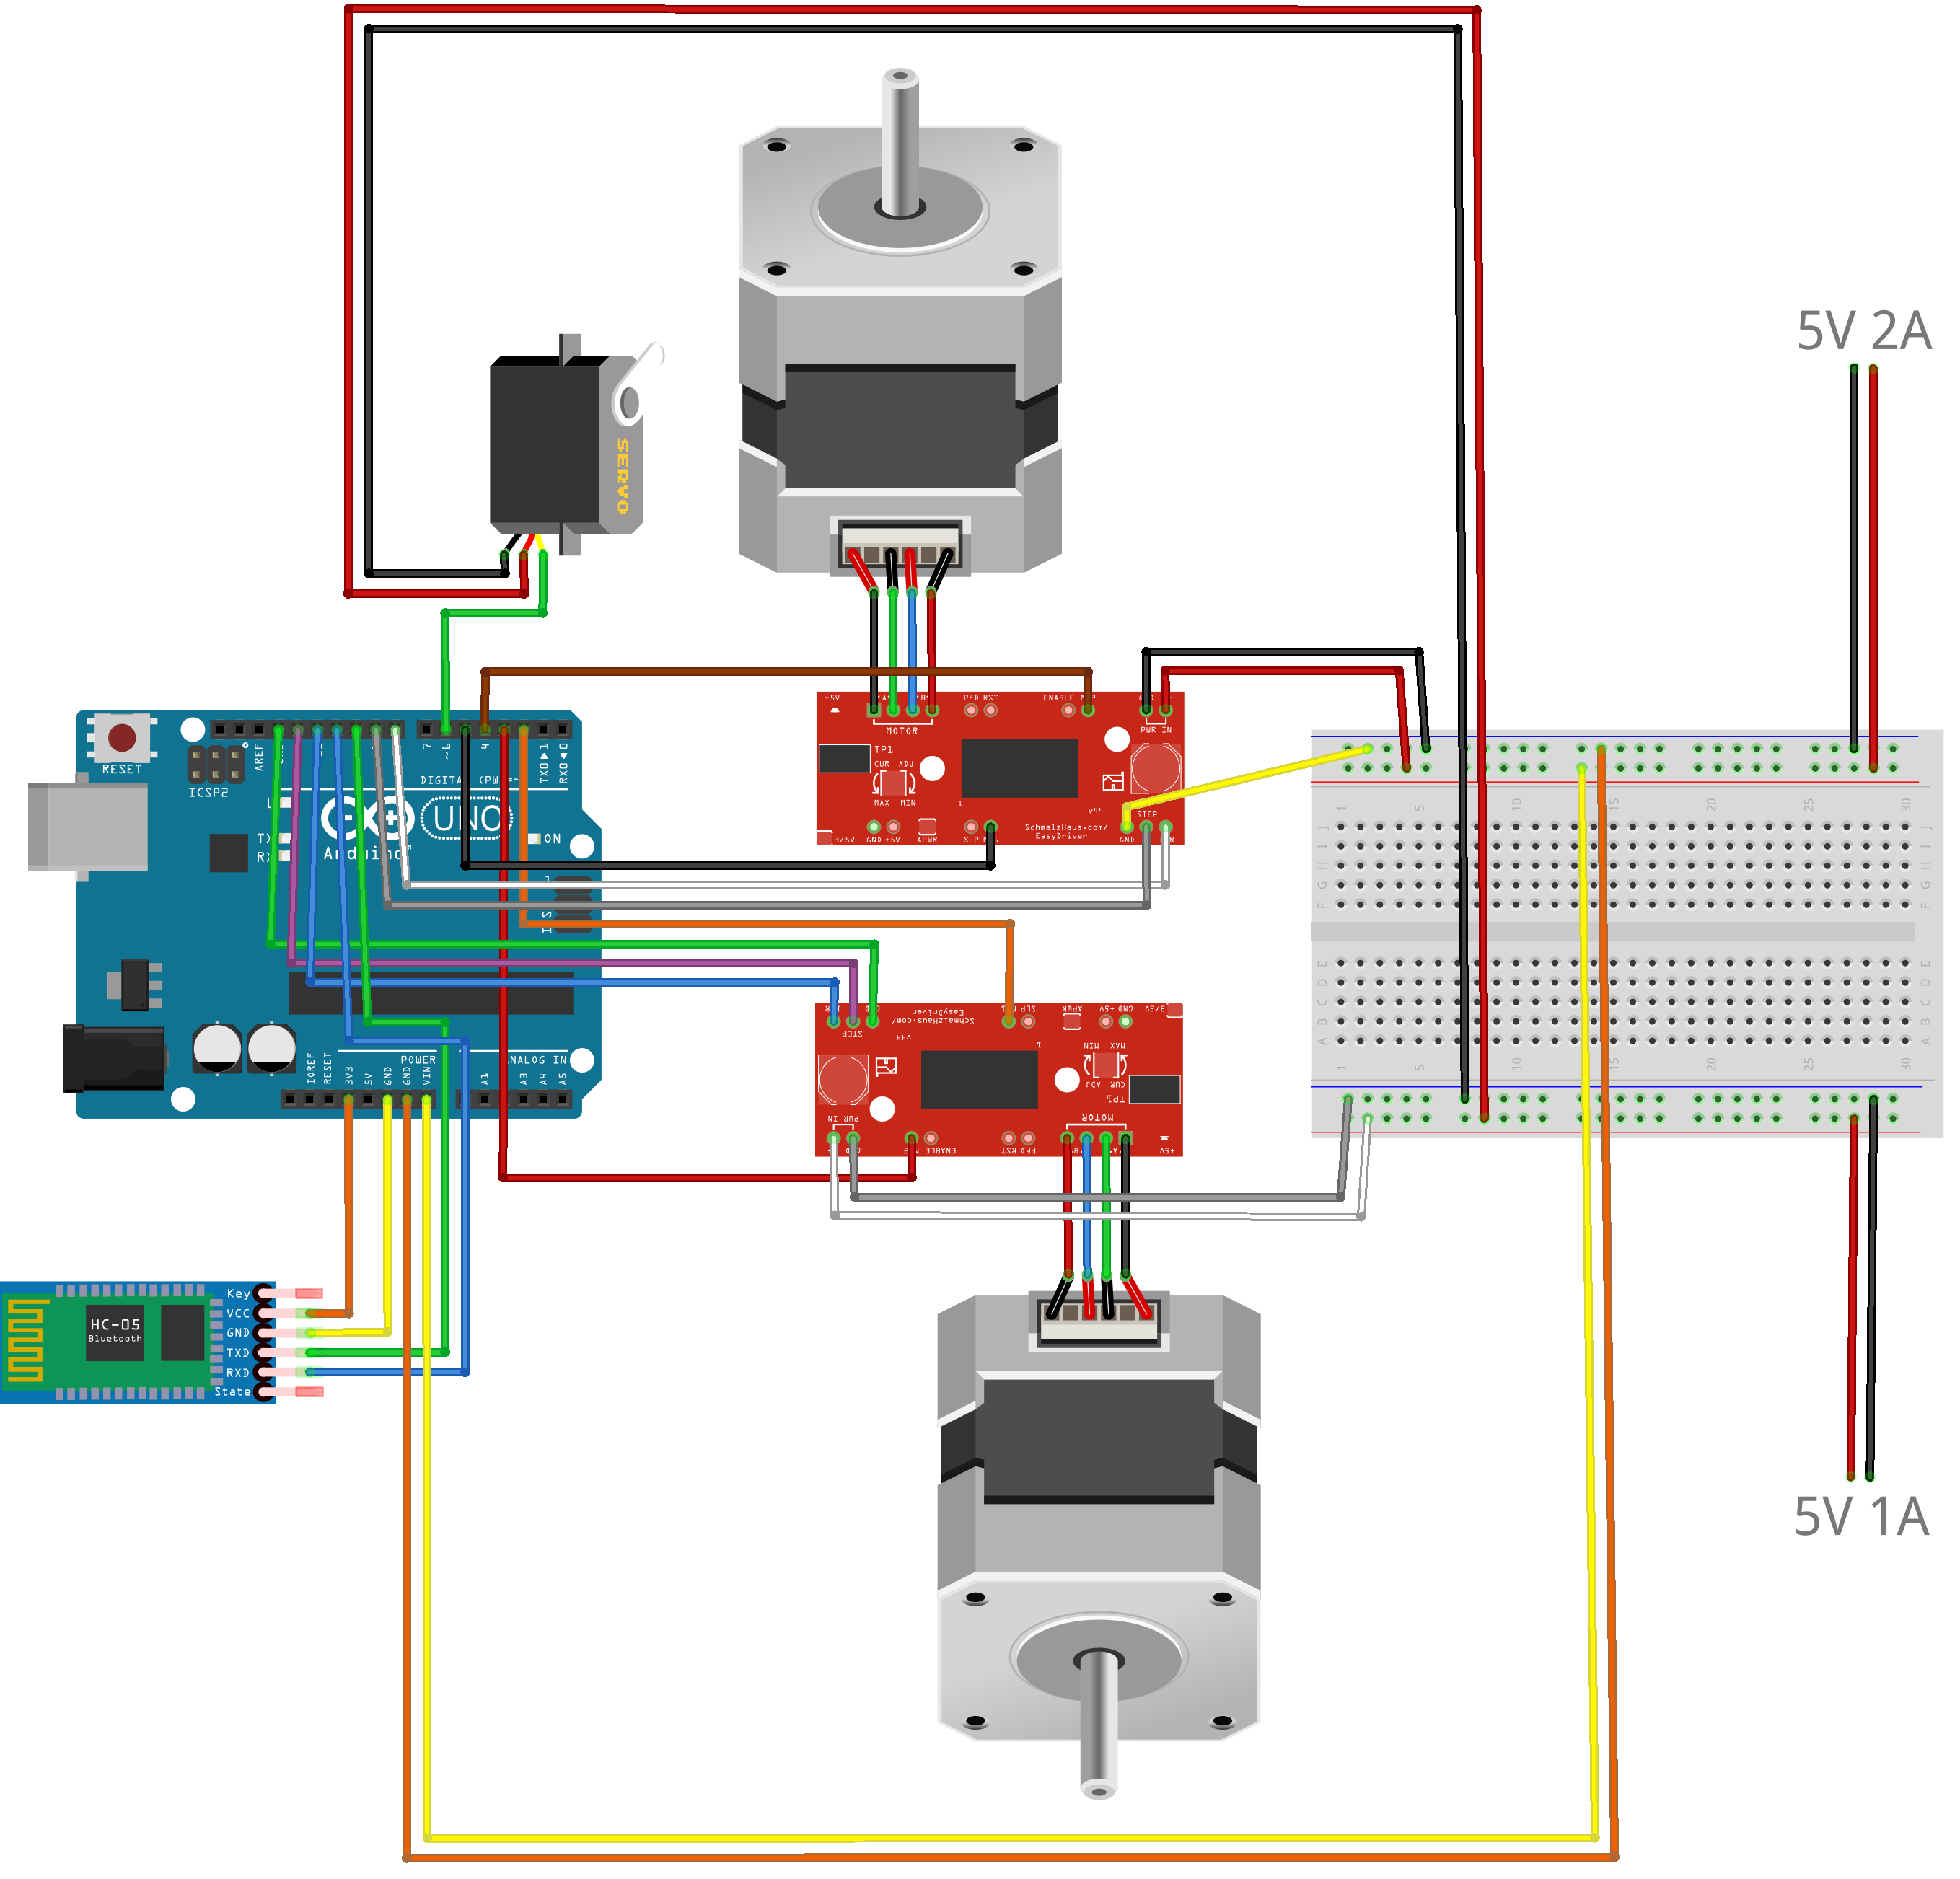
\includegraphics[scale=0.5]{RobotFritz}
	\caption{Diagrama de connexió dels components realitzada amb el programa Fritzing \cite{FritzingBib}.}
	\label{fig:connexio}
\end{figure}
\subsection{Programa Robot.ino}

S’ha creat un programa genèric amb la funció de llegir les ordres enviades des de l’ordinador. S’ha decidit fer d’aquesta manera per evitar la reprogramació constant de la placa a cada trajectòria i aconseguir així el control total del robot des de l’ordinador. 

La dinàmica de comunicació consisteix en rebre un missatge des de l’ordinador que conté 3 valors separats pel caràcter ‘,’ definit com el caràcter de separació. Aquests valors són: en primer lloc la posició del servo, que serà 1 si aquest ha d’estar dibuixant i 0 si s’ha d’aixecar. Els dos següents valors són la posició absoluta dels motors mesurada en passos, en primer lloc de la roda dreta i per acabar de l’esquerra. 

Tot seguit es fa una descripció del programa per entendre el seu funcionament. El programa complet està present a l’annex \ref{ArduinoProg}:

\subsubsection{Llibreries utilitzades}

El primer que cal fer és importar les llibreries que s’utilitzaran a l'executar el programa amb les següents comandes:

\begin{lstlisting}[style=Arduino]
#include <AccelStepper.h>
#include <MultiStepper.h>
#include <Servo.h>
#include <SoftwareSerial.h>
\end{lstlisting}

La primera llibreria AccelStepper \cite{guiadelallibreriaaccelstepper} permet enviar els senyals de control al driver per tal de moure cadascun dels motors, definint la velocitat i els passos que ha de realitzar. És una llibreria molt funcional pel control de motors pas a pas amb Arduino, tot i que no és possible moure els dos motors simultàniament amb aquesta llibreria. És per això que també s’utilitza la llibreria MultiStepper \cite{guiadelallibreriamultistepper}, que permet agrupar elements per tal de moure’ls alhora. Per fer-ho, com es veurà més endavant, es defineixen les posicions dels dos motors i aquests realitzaran un moviment constant controlant la velocitat de manera que finalitzaran el seu recorregut amb el mateix increment de temps, permetent així les trajectòries circulars. Aquestes dues llibreries no venen incorporades a l'entorn Arduino, però són igualment de codi lliure i es poden descarregar de la xarxa.

Les llibreries Servo i SoftwareSerial sí que s’inclouen en la descàrrega inicial del software Arduino i per tant no cal descarregar-les d’internet. La primera s’utilitza per controlar la posició del servomotor, mentre que la segona és l’encarregada d’establir la comunicació serial amb l’ordinador a partir del mòdul de Bluetooth. 

\subsubsection{Configuració}

Un cop incorporades les llibreries cal inicialitzar tots els paràmetres necessaris: 

\begin{itemize}
	\item Definició dels motors: 
	
	\begin{lstlisting}[style=Arduino]
	AccelStepper RodaDreta(1,9,8);
	AccelStepper RodaEsquerra(1,13,12);
	MultiStepper Robot;
	
	int VelocitatMax=500;
	int posicio[2];
	int pasdreta=0; 
	int pasesquerra=0;
	\end{lstlisting}
	
	
	Primerament es defineixen els motors per separat com objectes de la classe AccelStepper, on s’indica el tipus de control del motor (en aquest cas l’1 equival al control d’un motor bipolar a través d’un driver) i els pins als quals es connecten els pins d’STEP i Direcció de cadascun, entrades 9 i 8 pel motor dret i 13 i 12 per l’esquerre. Es defineix també l’objecte Robot de la classe MultiStepper al qual més endevant s’hi afegiran els dos motors. Després es defineixen variables que s’utilitzaran per definir els moviments: la velocitat màxima en steps/segon, una matriu amb la posició dels dos motors i la variable que definirà la posició de cada motor com el nombre absolut de passos que ha fet cada motor. 
	
	Amb els objectes ja definits, dins al bucle de configuració inicial (void setup()) es defineixen els pins 2, 3, 4 i 5 com sortides actives per activar així els senyals MS1 i MS2 dels drivers aconseguint d’aquesta manera el microstepping i multiplicant per 8 el nombre de passos del motor. Tot seguit s’afegeixen els dos motors de la classe AccelStepper al Robot que definirà el moviment conjunt dels dos motors i s’estableix la velocitat màxima dels dos motors. 
	
	\begin{lstlisting}[style=Arduino]
	pinMode(2, OUTPUT); 
	pinMode(3,OUTPUT);
	digitalWrite(2,HIGH);
	digitalWrite(3,HIGH);
	pinMode(4, OUTPUT);
	pinMode(5,OUTPUT);
	digitalWrite(4,HIGH);
	digitalWrite(5,HIGH);
	
	Robot.addStepper(RodaDreta);
	Robot.addStepper(RodaEsquerra);
	
	RodaDreta.setMaxSpeed(VelocitatMax);	
	RodaEsquerra.setMaxSpeed(VelocitatMax);
	\end{lstlisting}	
	\item Definició del servo:
	\begin{lstlisting}[style=Arduino]
	Servo boli;
	int up=0;
	int down=50;
	\end{lstlisting}
	
	Aquí es defineix l’objecte Boli de la classe Servo que controlarà la posició del servomotor. S’han definit les dues posicions que pot assolir, a 0 graus quan està aixecat i a 50 si està dibuixant. Al bucle de configuració es defineix el pin 6 com a sortida pel servomotor i la posició inicial es fixa en 0, per tant amb el retolador aixecat.
	\begin{lstlisting}[style=Arduino]
	Boli.attach(6);
	Boli.write(0);
	\end{lstlisting}
	
	\item SoftwareSerial:
	\begin{lstlisting}[style=Arduino]
	SoftwareSerial bluetooth(10,11);
	\end{lstlisting}
	
	Per acabar es defineix l’objecte Bluetooth de la classe SoftwareSerial que es connecta al pin 10 com RX de recepció de dades i a l’11 com TX de transmissió de dades. Aquesta connexió s’inicia al bucle de configuració amb la comanda: 
	\begin{lstlisting}[style=Arduino]
	bluetooth.begin(9600);
	\end{lstlisting}
	
	La comunicació es realitza a 9600 bps (bits per segon) ja que aquesta és la configuració per defecte del mòdul Bluetooth. 
	
	
\end{itemize}


\subsubsection{Bucle principal}

Aquest programa es basa en dues funcions que es criden seqüencialment, de manera que a l'acabar l’execució de la primera s’executi instantàniament la segona. Aquestes són la funció getSerialData() que, com el nom indica, s’encarrega de rebre i emmagatzemar les dades rebudes per Bluetooth, i la funció processData() que processa les dades preses i provoca l’acció dels motors seguint l’ordre rebuda. A l'acabar s’envia un missatge conforme la placa està llesta per rebre una nova ordre. 
\begin{lstlisting}[style=Arduino]
void loop() {
	getSerialData();
	delay(1);
	processData();
}
\end{lstlisting}
\begin{itemize}
	\item \textbf{getSerialData()}:
	
	El funcionament d’aquesta funció és molt senzill. El primer que avalua és si s’ha rebut un missatge per part de l’ordinador amb la funció bluetooth.available(). Si s’ha rebut es guarda com un String a la variable \emph{x}, i es crea una variable \emph{buff} que servirà per emmagatzemar caràcters. 
	
	\begin{lstlisting}[style=Arduino]
	void getSerialData(){
		if(bluetooth.available() > 0) {
			String x = bluetooth.readString();
			String buff="";
	\end{lstlisting}
	
	Tot seguit es recorre l’string rebut i guardat a la variable \emph{x} caràcter a caràcter per tal de separar-la per les comes, ja que aquest és el caràcter definit com a separador pel programa. Aquesta funció \emph{for} que recorre la cadena emmagatzema els caràcters llegits a la variable \emph{buff} fins a trobar el caràcter de separació ‘,’ i els guarda a la matriu text en la posició \emph{cnt} on \emph{cnt} és un comptador que augmenta en una unitat cada cop que es guarda un valor a la matriu text. D’aquesta manera s’inicia en \emph{cnt=0}, es guarda el primer valor quan està complet, s’incrementa \emph{cnt=1} i es guarda el segon valor complet, es torna a incrementar \emph{cnt=2} per emmagatzemar el tercer i últim valor i es reinicia el valor del comptador \emph{cnt} abans d’acabar el for. 
	
	\begin{lstlisting}[style=Arduino]
			for (int i=0; i<x.length();i++){
				String caracter="";
				caracter=caracter+x[i];
				if (caracter!=","){
					buff=buff+x[i];
				}
				else {
					int y=buff.toInt();
					text[cnt]=y;
					buff="";
					if (cnt<3){
						cnt+=1;
					}
					if (cnt==3){
						cnt=0;
					}
				}
			}
			Rebut=true;
			delay(1);    
		}
	}
	\end{lstlisting}
	
	Per acabar, es canvia el valor de la variable booleana \emph{Rebut} a \emph{True}, de manera que així pugui començar a treballar la funció processData() un cop llegit tot el missatge. 
	
	\item \textbf{processData()}:
	
	Un cop rebut i llegit el missatge només cal processar aquesta informació i enviar les ordres adients als motors amb la següent funció:
	
	\begin{lstlisting}[style=Arduino]
	void processData(){
		if (Rebut==true){
			if (text[0]==0 and Boli.read()!=up){
				Boli.write(up);
				delay(300);
			}
		else if (text[0]==1 and Boli.read()!=down){
			Boli.write(down);
			delay(300);
		}
		posicio[0]=-text[1];
		posicio[1]=text[2];
		Robot.moveTo(posicio);
		Robot.runSpeedToPosition();
		bluetooth.println("Ready");
		Rebut=false; 
		}
	}
	\end{lstlisting}
	
	En primer lloc, només s’executa la funció si la variable \emph{Rebut} val \emph{True} i, per tant, s’ha rebut un missatge complet. Un cop dins la funció es llegeixen els 3 valors de la matriu text, de manera que, si el primer valor (\emph{text[0]}) val 0 i el retolador està en posició de dibuix, s’aixeca, i si val 1 i està aixecat es baixa. Es pot observar que després de l’acció del servo s’atura el programa 300 ms per tal d’assegurar la posició del retolador abans de començar amb el nou moviment. A partir d’aquí, es guarden els dos valors a una matriu que conté la posició dels motors, tenint en compte que es canvia el signe de la posició del motor dret per tal d’aconseguir que girin en el mateix sentit , ja que un motor està situat a la inversa de l’altre. Aquesta matriu s’envia als drivers amb les ordres moveTo() i runSpeedToPosition() de la classe MultiStepper que realitzaran els moviments esperats dels motors. 
	
	Per acabar s’envia un missatge de retorn a l’ordinador amb la paraula “Ready” per tal de continuar amb l’execució de la següent ordre. 
	
	
\end{itemize}

\section{Bluetooth: Com es comuniquen l'ordinador i el robot?}

És de vital importància establir una comunicació bidireccional entre l’ordinador i l’Arduino per tal de poder controlar el robot i programar les noves traçades. Hi ha moltes maneres d’establir aquesta comunicació: per cable, a través d’una xarxa wifi, amb una targeta de memòria... Cadascuna té els seus avantatges i desavantatges i, després d’analitzar-les s’ha decidit utilitzar un dispositiu Bluetooth. En aquest apartat es presentarà el mòdul HC-05 encarregat d’establir aquesta comunicació.

\begin{figure}[H]
	\centering
	
\includegraphics[scale=0.03]{BluetoothLogo}
	\caption{Logo de la tecnologia Bluetooth.}
	\label{fig:BTlogo}
\end{figure}

\subsection{Mòdul HC-05}

Els dispositius Bluetooth tenen la capacitat de connectar-se entre si a partir d’ones de radiofreqüència, eliminant així cables o connectors físics. Aquesta comunicació es realitza a una freqüència entre 2,4 i 2,48 GHz i permet crear una xarxa sense fils entre diferents dispositius els quals es poden enviar dades i compartir informació. Aquestes xarxes es regeixen per un element dominant o master i una sèrie d’elements esclaus o slaves. En aquest cas com a  element master actua l’ordinador, i l’Arduino actua d’esclau mitjançant el mòdul HC-05 \cite{HC05Bib}. Aquestes xarxes poden tenir un abast de 10 metres aproximadament, tot i que n’hi ha que poden arribar fins a 100 m. 

\begin{figure}[H]
	\centering
	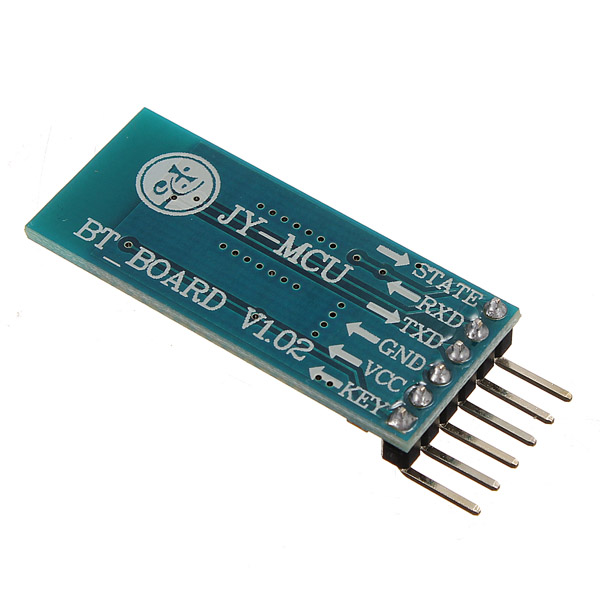
\includegraphics[scale=0.3]{HC05}
	\caption{Mòdul HC-05.}
	\label{fig:HC05}
\end{figure}

El mòdul HC-05 pot actuar com a master o com a slave, però en aquest cas s’utilitza en la seva configuració per defecte en mode slave, ja que l’ordinador pot actuar com a master. Aquest mòdul és molt utilitzat en projectes Arduino gràcies a la seva fàcil connexió i configuració. Presenta 6 pins diferents tot i que només se n’utilitzen 4 per connectar-lo. Els pins Vcc i GND són els encarregats del subministrament de corrent i cal connectar-los als pins de 3,3 V i GND respectivament. Cal afegir que el fabricant recomana no connectar el mòdul a més de 3,6 V per no fer-lo malbé i per això s’utilitza el pin de 3,3 V. Per altra banda, els pins RX i TX són els encarregats de la recepció i transmissió de dades. S'encarreguen d'establir la comunicació desitjada i, com s’ha explicat a l’apartat \ref{sec:connexio}, es connecten als pins 10 i 11 de la placa. 

Per altra banda existeixen els pins KEY i STATE que no s’utilitzaran en aquesta aplicació. El pin STATE només reflexa la situació en la que es troba el mòdul, i en quin mode de funcionament treballa, mentre que el pin KEY permet accedir a les comandes AT de programació del propi xip del mòdul. Aquesta programació permet canviar el mètode de funcionament, com ara passar de slave a master, canviar la velocitat de transmissió o Baud rate, o canviar el codi d’emparellament utilitzat per emparellar el mòdul amb qualsevol altre dispositiu. Per defecte aquest treballa com a esclau, a una velocitat de 9600 baud/s, a la mateixa a la que s’ha programat l’Arduino, i el codi d’accés és 1234. No s’ha canviat cap d’aquests paràmetres ja que no va ser necessari. 

Per acabar, també disposa d’un díode LED que indica l’estat de la connexió del mòdul, que mostrarà si el mòdul està correctament connectat. Mentre no es connecta amb l’ordinador aquest parpelleja dues vegades per segon mentre que si la connexió s’ha establert,  aquest ho fa un cop cada dos segons. 


\section{Aplicació: Com es controla?}

Per tal de millorar l’experiència de l’usuari i no haver d’utilitzar el terminal de comandes de Python, fet que pot semblar complicat per persones no familiaritzades amb la programació, s’ha creat una aplicació bàsica i senzilla per tal de controlar el propi robot. Es basa en un petit programa que ofereix dos mètodes de funcionament: a partir d’un arxiu .txt creat prèviament en Inkscape seguint les instruccions de l’apartat \ref{sec:ManualInk}, o escrivint pas a pas les ordres que es volen donar al robot i visualitzant-les abans.
Aquesta aplicació d’escriptori s’ha crear amb el mòdul que incorpora Python per creat interfícies GUI anomenat Tkinter que s’explicarà més detalladament a les següents línies. 

\subsection{Tkinter}
Tkinter és un mòdul de Python que permet als usuaris crear GUI’s. Una GUI és una Interfície Gràfica d’Usuari que proporciona a l’usuari un entorn visual senzill per interaccionar amb el programa a partir d’un seguit d’objectes i imatges que representen les diferents opcions disponibles al programa principal. L’objectiu d’aquesta és establir la comunicació entre l’usuari i el robot de manera fàcil i entenedora, per fer-lo accessible per a qualsevol interessat. 

Les GUI creades amb Tkinter es basen en finestres o espais (frames) i objectes (widgets) que el programador pot col·locar al seu gust. Els frames són els espais que ocuparan després els objectes, les finestres visibles per l’usuari, i dins d’aquests es creen els objectes o widgets, que poden ser entrades de text, botons, imatges, gràfics, entre d’altres. Els frames són els encarregats de donar forma al programa i organitzar els propis widgets, mentre que aquests estableixen la comunicació amb l’usuari, permetent la interacció per tal de controlar el programa i decidir les accions a emprendre. 

\subsection{Aplicació}
Per aquest projecte, com s’ha explicat abans, s’ha creat una GUI bàsica per interaccionar amb el robot des de l’ordinador. El programa s’ha organitzat en finestres per facilitar aquesta interacció, tenint 3 finestres diferents: la pàgina inicial on es triarà el mètode de funcionament, la part dedicada a dibuix de trajectòries creades prèviament amb Inkscape i una última finestra on l’usuari pot dibuixar pas a pas la trajectòria que desitgi introduint una a una totes les comandes.

Les llibreries que utilitza són les següents:

\begin{python}
	import math
	
	import Tkinter as tk
	import ttk
	
	import turtle
	import Draw
	import RobotMoveBT
\end{python}

La llibreria math s'utilitza per realitzar operacions matemàtiques, igual que als altres programes. La llibreria Tkinter \cite{TkinterBib}, com s’ha explicat a l’apartat anterior, és el motor de creació de la GUI i la llibreria Turtle \cite{turtleBib}, que permet crear dibuixos i gràfiques i que s’utilitza per tal de representar les trajectòries introduïdes. Per altra banda també s’utilitza l’arxiu Draw.py que s’explicarà a l’apartat \ref{sec:Draw} i que permet dibuixar aquestes ordres utilitzant la llibreria Turtle a la pantalla de la GUI.  Per últim incorpora també l’arxiu RobotMoveBT.py presentat a l’apartat \ref{sec:robotmoveBT} que s’encarrega de moure el robot. 

El programa està estructurat en quatre classes, tres que defineixen cadascuna d’aquestes finestres que es mostren a l’usuari, i una classe mare que inicia el programa i organitza les altres. Aquesta última és la classe TFM, la classe principal, i és l’única que es crida a l'executar el programa, i té la funció de crear els frames corresponents a les altres classes. No té cap pàgina ni objecte associat, només serveix com a inicialització i com a motor per organitzar les altres classes, ja que per canviar d’una finestra a un altre s’utilitza la comanda show\_frame() definida aquí. El codi de definició d’aquesta classe és el següent:

\begin{python}
	class TFM(tk.Tk):
	
		def __init__(self, *args, **kwargs):
		
			tk.Tk.__init__(self, *args, **kwargs)
			
			tk.Tk.wm_title(self, "TFM Josep Marti")
			
			
			container = tk.Frame(self)
			container.pack(side="top", fill="both", expand = True)
			container.grid_rowconfigure(0, weight=1)
			container.grid_columnconfigure(0, weight=1)
			
			self.frames = {}
			
			for F in (StartPage, Inkscape, Manual):
			
				frame = F(container, self)
				
				self.frames[F] = frame
				
				frame.grid(row=0, column=0, sticky="nsew")
			
			self.show_frame(StartPage)
	
	def show_frame(self, cont):
	
	frame = self.frames[cont]
	frame.tkraise()
\end{python}

Primer s’inicialitza la GUI amb la comanda Tk.\_\_init\_\_, després es defineix el títol del programa que apareix al marc superior esquerre de la finestra amb la comanda Tk.wm\_title() i es configuren els frames corresponents a les finestres ja esmentades. S’inicialitza l’aplicació mostrant primer la pàgina inicial amb la funció show\_frame(StartPage), que es crea tot seguit. 

Un cop ja definits tots els frames que s’utilitzen, es creen les finestres que es mostraran a l’usuari, començant per la pàgina principal sota el nom de StartPage. El primer pas és inicialitzar el frame amb la comanda tk.Frame.\_\_init\_\_(self, parent, controller), que el que fa és inicialitzar la finestra amb la configuració definida a la classe mare inicial. A partir d’aquí només es creen i s’empaqueten els diferents objectes o widgets a la finestra. En aquest cas només hi ha un títol que correspon a la pregunta “Com vols dibuixar?” i dos botons que canvien a les dues altres finestres. Per tal de mostrar aquests objectes a la pantalla hi ha 3 mètodes diferents, en aquest cas s’utilitza el mètode .pack(), que permet implementar els elements de manera simple automàticament. També existeix el mètode .grid() que s’utilitzarà a l’última pàgina, i permet l’organització dels elements en files i columnes, i per últim el mètode .place() que utilitza les coordenades globals de la pàgina i que no s’ha utilitzat en aquest projecte. 

D’aquesta manera, la pàgina inicial és la següent:

\begin{figure}[H]
	\centering
	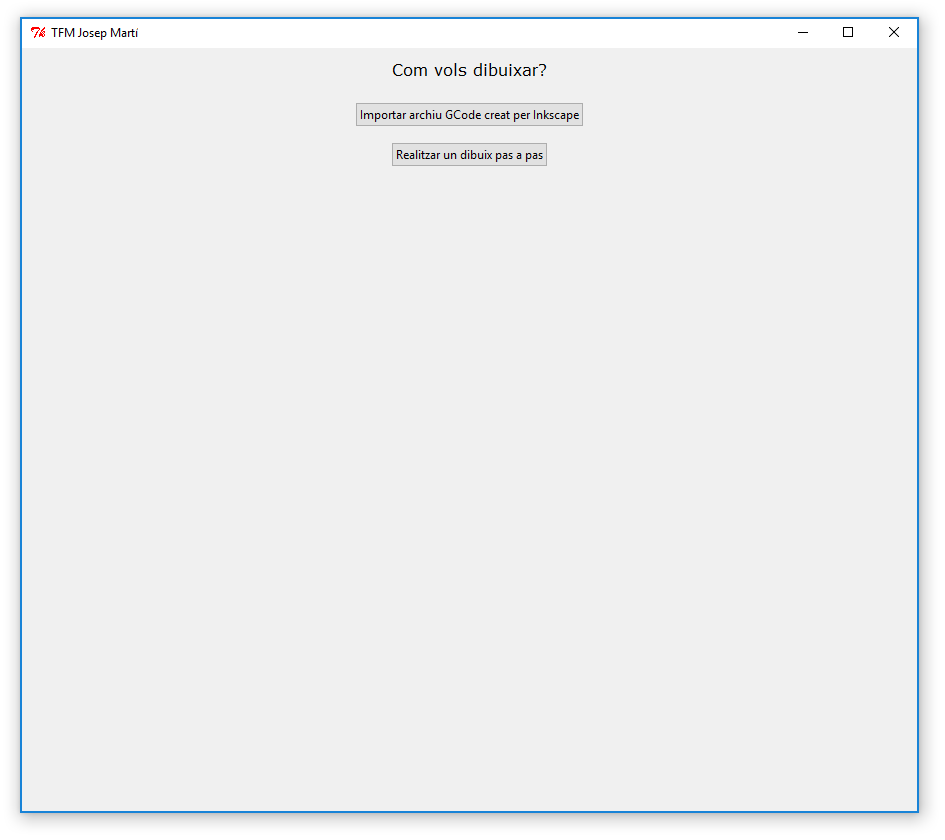
\includegraphics[scale=0.9]{StartPage}
	\caption{Pàgina inicial.}
	\label{fig:StartPage}
\end{figure}

El seu codi associat és aquest:

\begin{python}
	class StartPage(tk.Frame):
	
	def __init__(self, parent, controller):
	tk.Frame.__init__(self,parent)
	label = tk.Label(self, text="Com vols dibuixar?", font=LARGE_FONT)
	label.pack(pady=10,padx=10)
	
	button = ttk.Button(self, text="Importar archiu GCode creat per Inkscape",
	command=lambda: controller.show_frame(Inkscape))
	button.pack(pady=10,padx=10)
	
	button2 = ttk.Button(self, text="Realitzar un dibuix pas a pas",
	command=lambda: controller.show_frame(Manual))
	button2.pack(pady=5,padx=5)
\end{python}

La següent pàgina es crea a partir de la classe Inkscape i és la finestra que permet a l’usuari dibuixar a partir d’un fitxer .txt creat prèviament amb Inkscape i que conté el GCode associat a la trajectòria. Per tal de crear-lo, cal seguir les instruccions de l’apartat \ref{sec:ManualInk}. El seu funcionament és molt simple, s’ha incorporat una cel·la d’entrada de text en la qual s’haurà d’escriure el nom del fitxer sempre acompanyat de la seva extensió (\emph{.txt}). Cal remarcar que, perquè el programa funcioni, cal desar l’arxiu a la mateixa carpeta des d’on s’executa el programa, ja que sinó no serà capaç de trobar-lo.

A partir d’aquí es presenten 3 opcions: Dibuixar, Previsualitzar i Tornar a l’inici.  Aquestes opcions es representen per botons i cadascun té un funció associada. La primera, Dibuixar, envia al robot l’ordre de dibuixar la trajectòria que conté el document amb la funció GCode de l’arxiu "RobotMoveBT.py". Un cop començada la representació no es pot realitzar cap altre operació fins que aquesta acabi. La funció Preview per representar la trajectòria del fitxer a la pantalla, crida l’arxiu "Draw.py" i a partir de la llibreria Turtle de Python crea una representació virtual del que el robot dibuixarà. Per acabar, l’opció Tornar a l’inici esborra la representació i torna a la pàgina inicial. 

Per tal de fer la representació del dibuix, s’ha utilitzat un “canvas”, que és un espai reservat per una figura. En aquest cas, s’ha utilitzat aquest espai per iniciar la llibreria Turtle sota el nom de turtle1. L’aspecte d’aquesta pàgina és el següent:

\begin{figure}[H]
	\centering
	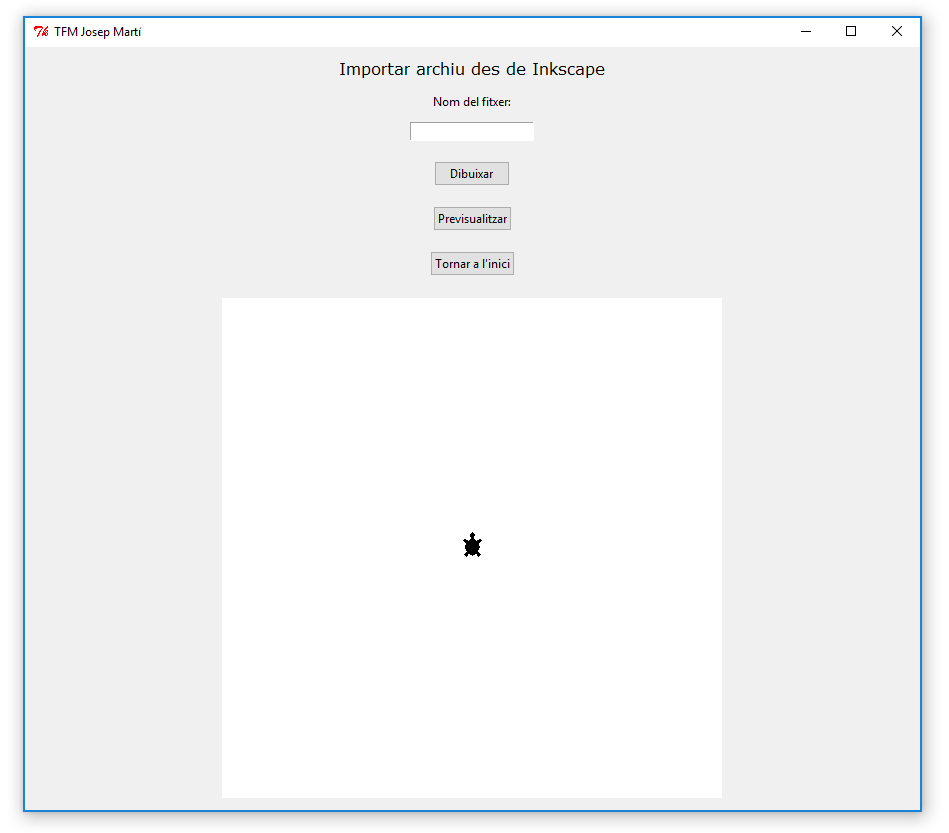
\includegraphics[scale=0.9]{InkPage}
	\caption{Pàgina de dibuix a partir d'Inkscape.}
	\label{fig:InkPage}
\end{figure}

I el codi el següent:

\begin{python}
	class Inkscape(tk.Frame):
	
	def __init__(self, parent, controller):
	nomfitxer=tk.StringVar(None)
	
	tk.Frame.__init__(self, parent)
	
	
	label = tk.Label(self, text="Importar archiu des de Inkscape", font=LARGE_FONT).pack(pady=10,padx=10)
	
	label2=tk.Label(self, text='Nom del fitxer:').pack()
	
	fitxer=tk.Entry(self, textvariable=nomfitxer).pack(pady=10,padx=10)
	
	button1 = ttk.Button(self, text="Dibuixar",command=lambda:Dibuixa(self)).pack(pady=10,padx=10)
	
	button2 = ttk.Button(self, text="Previsualitzar",command=lambda:Preview(self)).pack(pady=10,padx=10)
	
	button3 = ttk.Button(self, text="Tornar a l\'inici",command=lambda: back(self)).pack(pady=10,padx=10)
	
	canvas = tk.Canvas(self, width=500, height=500)
	canvas.pack(pady=10,padx=10)
	
	turtle1 = turtle.RawTurtle(canvas)
	turtle1.shape("turtle")
	turtle1.setheading(90)
	turtle1.radians()
	
	def Dibuixa(self):
	nom=nomfitxer.get()
	RobotMoveBT.GCode(nom)
	
	def Preview(self):
	nom=nomfitxer.get()
	Draw.previsualitzaFitxer(turtle1,nom)
	
	def back(self):
	turtle1.reset()
	turtle1.setheading(math.pi/2.0)
	controller.show_frame(StartPage)
\end{python}

Per acabar, en la tercera i última pàgina es presenta l'oportunitat per l’usuari de crear pas a pas el seu GCode. La idea d’aquesta finestra és permetre dibuixar i dissenyar les trajectòries del robot directament des de l’aplicació sense utilitzar programes externs com l’Inkscape. Com la resta de pàgines es defineix com una classe dins la classe mare sota el nom de Manual. 

La disposició dels objectes que apareixen és la següent:

\begin{figure}[H]
	\centering
	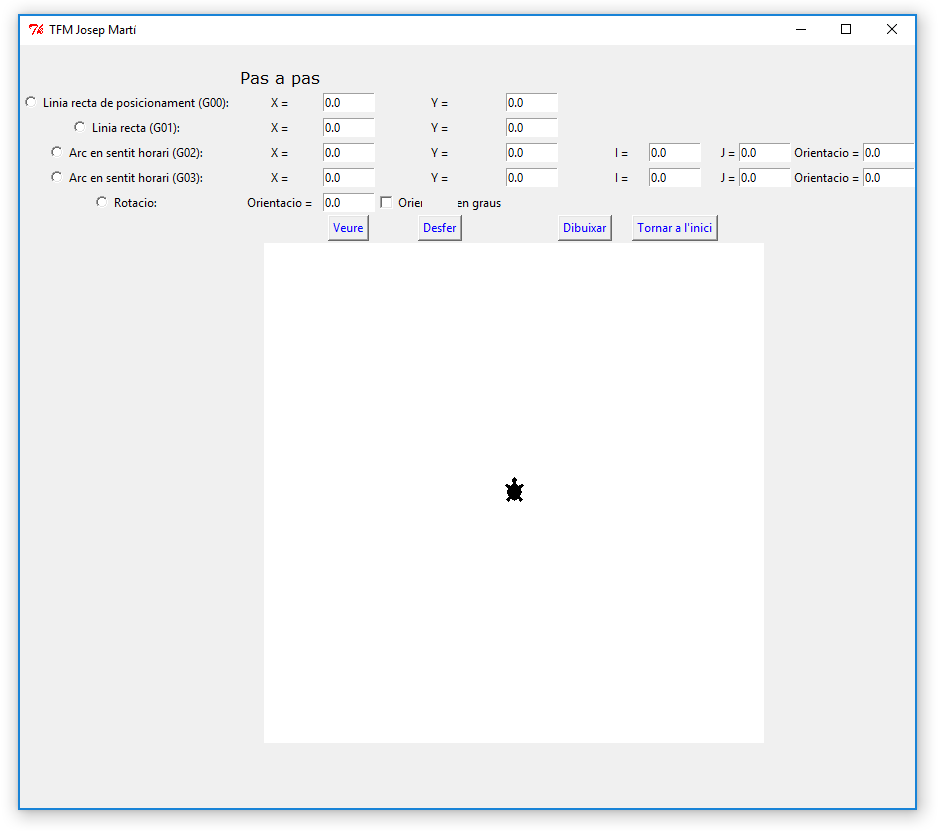
\includegraphics[scale=0.9]{ManualPage}
	\caption{Pàgina de dibuix manual.}
	\label{fig:ManualPage}
\end{figure}

Com es pot observar, s’ha creat una sèrie de 5  “radio buttons” que són botons de selecció els quals només permeten que un estigui activat. Cadascun correspon a un dels moviments programats, G00, G01, G02, G03 i G01 de rotació. Associades a aquests botons hi ha les entrades de text que cal omplir per definir el moviment a la mateixa línia, que són les mateixes que defineix el GCode creat amb Inkscape: les coordenades X i Y del punt de destí, les cordenades Xc i Yc del centre de gir en el cas de les comandes G02 i G03 i l’orientació del robot a l'acabar el moviment també per les comandes G02 i G03 i per la comanda G01 de rotació. S’ha incorporat també una “checkbox” per definir, si cal, si l’orientació està calculada en graus o en radians (per defecte sempre funciona en radians). Tot seguit s'exposa el codi de la línia d'objectes que representen totes les variables necessaries per realitzar una traçada circular amb la comanda G02:

\begin{python}
	#G02
	radioG=tk.Radiobutton(self,text='Arc en sentit horari (G02): ', value='G02', variable=ordre).grid(row=7,column=0)
	labelG02X=tk.Label(self, text='X =').grid(row=7,column=2)
	entryG02X=tk.Entry(self, textvariable=G02X, width=8).grid(row=7,column=3)
	labelG02Y=tk.Label(self, text='Y =').grid(row=7,column=5)
	entryG02Y=tk.Entry(self, textvariable=G02Y, width=8).grid(row=7,column=6)
	labelG02I=tk.Label(self, text='I =').grid(row=7,column=8)
	entryG02I=tk.Entry(self, textvariable=G02I, width=8).grid(row=7,column=9)
	labelG02J=tk.Label(self, text='J =').grid(row=7,column=11)
	entryG02J=tk.Entry(self, textvariable=G02J, width=8).grid(row=7,column=12)
	labelG02A=tk.Label(self, text='Orientacio =').grid(row=7,column=14)
	entryG02A=tk.Entry(self, textvariable=G02A, width=8).grid(row=7,column=15)
\end{python}

A partir d’aquí s’han incorporat els botons d’acció i, com a la finestra Inkscape explicada anteriorment, un “canvas” amb la representació de la trajectòria introduïda. Hi apareixien quatre botons diferents: Visualitzar, Desfer, Dibuixar i Tornar a l’inici. Un cop introduïda una ordre, cal representar-la amb el botó Visualitzar per comprovar que és la desitjada. Un cop vista, es pot seguir dibuixant afegint comandes o manar al robot dibuixar la representació vista al canvas. L’opció Desfer permet esborrar l’últim moviment programat. Un cop el robot estigui en moviment caldrà esperar que acabi tot el moviment, ja que la interrupció del mateix no està programada. El codi corresponent a la programació dels botons i la definició de les seves funcions associades és el següent:

\begin{python}
	#Botons
	buttonDibuixar=tk.Button(self, text='Dibuixar', fg='blue', command=lambda:Dibuixar(self)).grid(row=20,column=7)
	buttonVeure=tk.Button(self, text='Veure', fg='blue', command=lambda: Veure(self)).grid(row=20,column=3)
	buttonUndo=tk.Button(self, text='Desfer', fg='blue', command=lambda: undo(self)).grid(row=20,column=5)
	buttonTorna=tk.Button(self, text='Tornar a l\'inici', fg='blue', command=lambda:back(self)).grid(row=20,column=9)
	
	canvas = tk.Canvas(self, width=500, height=500)
	canvas.grid(row=25,column=1,columnspan=12)
	
	turtle1 = turtle.RawTurtle(canvas)
	turtle1.shape("turtle")
	turtle1.setheading(90)
	turtle1.radians()
	
	label1=tk.Label(self, text='          ').grid(row=11,column=5)
	
	
	
	
	def Dibuixar(self):
	Draw.dibuixaLlista()
	
	
	def Veure(self):
	print ordre.get()
	tria=ordre.get()
	if tria == 'G00':
	x=G00X.get()
	y=G00Y.get()
	Draw.dibuixG00(turtle1,x,y)
	
	elif tria == 'G01':
	x=G01X.get()
	y=G01Y.get()
	Draw.dibuixG01(turtle1,x,y)
	
	elif tria == 'G02':
	x=G02X.get()
	y=G02Y.get()
	i=G02I.get()
	j=G02J.get()
	angle=G02A.get()
	graus=checkBox1.get()
	if graus == True:
	angle= (angle*math.pi)/180
	else:
	pass
	print (x, y, i , j, angle)
	Draw.dibuixG02(turtle1,x,y,i,j,angle)
	
	elif tria == 'G03':
	x=G03X.get()
	y=G03Y.get()
	i=G03I.get()
	j=G03J.get()
	angle=G03A.get()
	graus=checkBox1.get()
	if graus == True:
	angle= (angle*math.pi)/180
	else:
	pass
	Draw.dibuixG03(turtle1,x,y,i,j,angle)
	
	elif tria == 'apuntar':
	angle=RA.get()
	graus=checkBox1.get()
	if graus == True:
	angle= (angle*math.pi)/180
	else:
	pass
	Draw.dibuixapuntar(turtle1,angle)
	
	else:
	pass
	
	def undo(self):
	Draw.desfer(turtle1)
	
	
	def back(self):
	turtle1.reset()
	turtle1.setheading(math.pi/2.0)
	controller.show_frame(StartPage)
\end{python}

Es pot observar que en aquest cas s’ha utilitzat el mètode .grid() per organitzar els objectes al frame, ja que d’aquesta manera és més fàcil ordenar-los en files i columnes per tal que tot quedi alineat i al seu lloc.

\subsection{Draw.py} \label{sec:Draw}

Aquest arxiu s’ha creat per tal de calcular i realitzar la representació de les ordres a l’entorn de Python Turtle. Aquest és un mòdul que formava part del llenguatge de programació Logo creat per Wally Feurzig i Seymour Papert el 1966 i permet crear imatges amb un punter amb forma de tortuga i d’aquí ha heretat el nom de \emph{turtle}. Aquest obeeix les comandes introduïdes al Python dibuixant rectes i arcs de circumferència igual que el robot i s’ha utilitzat perquè tenen un mètode de funcionament similar. La representació és una aproximació a la representació real i a escala, ja que a la vida real les ordres es representen en mil·límetres mentre que, a la pantalla, es representen en píxels. La intenció d’aquest mòdul és donar una aproximació visual del futur resultat del robot per tal de comprovar què s’està dibuixant abans de començar. El codi del programa està present a l'annex \ref{PyDraw}. 

S'han definit les funcions correspoents a cada moviment possible del robot, les funcions: G00, G01, G02, G03 i G01 de rotació. Les comandes de la llibreria \emph{turtle} que ho fan possible són les següents:
\begin{itemize}
	\item turtle.penup(): Defineix la posició posició inactiva del retolador, quan aquest està aixecat i no dibuixa sobre el paper. Indica que els moviments que realitza la tortuga no quedaran representats. 
	
	\item turtle.pendown(): També defineix la posició del retolador però, al contrari que l'anterior, els moviments de la tortuga quedaran representats al canvas. En aquest cas la posició del retolador és activa i, per tant, dibuixa sobre el paper.
	
	\item turtle.setheading($angle$): Orientació de la tortuga a la direcció de l'angle introduït. Igual que la funció G01 de rotació, només rota sobre si mateixa sense desplaçar-se. 
	
	\item turtle.goto($x_{1},y_{1}$): Aquesta comanda mou la tortuga en línia recta des del punt on es trova fins a les coordenades desitjades ($x_{1},y_{1}$). És l'equivalent a la funció G00 i G01 del GCode i la representació de les traçades vindrà definida per la posició del retolador.
	
	\item turtle.circle($radi,angle$): És la funció utilitzada per dibuixar arcs de circumferència, igual que les comandes G02 i G03 del GCode. A diferència de les ordres G02 i G03 creades a Inkscape, les variables necessàries per definir el moviment són el radi i l'angle de gir en comptes de les coordenades de destí i del centre de gir. El sentit de gir, la diferència entre G02 (horari) i G03 (antihorari), es defineix amb el signe del radi, essent positiu pel sentit horari i negatiu per l'antihorari. 
\end{itemize}

Amb aquestes comandes és molt fàcil definir els moviments de la tortuga igual que els del robot. Per les comandes G00 i G01 només es calcula la direcció angular del punt de destí per orientar així la tortuga i realitzar un moviment en línia recta. A diferència del GCode creat per l'Inkscape, en aquest cas no cal realitzar una operació G01 de rotació prèvia a les operacions G01, ja que la pròpia comanda ja té en compte aquest canvi d'orientació i el realitza automàticament. Per altra banda, per les comandes G02 i G03, només cal calcular el radi de gir i l'angle de la mateixa manera que ho fa el programa "RobotMoveBT.py", i la diferència entre ells és el signe del radi de gir, positiu pel G02 i negatiu pel G03. 

Aquest programa també crea una llista de llistes anomenada \emph{moviments} que emmagatzema tots els moviments que s'han representat al canvas per després poder enviar les comandes ordenades al robot. Cada cop que s'executa una funció de dibuix al canvas s'afegeix una llista a la llista \emph{moviments} que conté, en primer lloc, el nom del moviment (G00, G01, G02, G03 o apuntar) i després els valors de les variables que defineixen el moviment. A partir d'aquesta llista, amb la funció \emph{dibuixaLlista()}, s'envien al robot cadascuna de les ordres de la llista per realitzar el dibuix. La funció \emph{previsualitzaFitxer()} serveix per representar la trajectòria definida en un arxiu creat amb Inkscape. 


